% OARF — Online Anchor-Robust Forecasting under Economic Regime Shift
% Submission variant for: International Journal of Forecasting (Elsevier)
%
% This file is the ANONYMIZED MANUSCRIPT for double-anonymized review: it must
% contain no author names, affiliations, or other identifying information (see
% titlepage_ijf.tex for the companion title page, submitted as a separate file
% per the journal's double-anonymized review instructions). Built on Elsevier's
% elsarticle.cls with the `authoryear` option so in-text citations render as
% "Author (Year)" per the journal's reference style; the body, floats, algorithm
% and \cite commands are otherwise unchanged from manuscript.tex.
%
% Compile with: pdflatex manuscript_ijf && bibtex manuscript_ijf \
%   && pdflatex manuscript_ijf && pdflatex manuscript_ijf

\documentclass[authoryear,preprint,12pt]{elsarticle}

% We deliberately keep the default OT1 text encoding so the body is set in the
% Computer Modern *Type-1* (vector) fonts that ship with a base TeX Live
% install. Loading [T1]{fontenc} without the lmodern or cm-super Type-1 EC
% fonts forces a bitmap Type-3 fallback for the running text, which renders as
% fuzzy/garbled glyphs in some PDF viewers; OT1 + cmap + glyphtounicode avoids
% that while still producing searchable, copy-pasteable ligatures.
\usepackage[utf8]{inputenc}
\usepackage{cmap}            % searchable/copyable ligatures
\input{glyphtounicode}
\pdfgentounicode=1
\usepackage{amsmath,amssymb,amsthm,bm}
\usepackage{graphicx}
\usepackage{booktabs}
\usepackage{array}
\usepackage{multirow}
\usepackage{caption}
\usepackage{subcaption}
\usepackage{xcolor}
\usepackage{enumitem}
\usepackage{algorithm}
\usepackage{algpseudocode}
\usepackage[section]{placeins}  % keep floats within their section
\usepackage[hidelinks]{hyperref}
\usepackage{xurl}               % allow long URLs to break across lines

\graphicspath{{../figures/}}

\theoremstyle{plain}
\newtheorem{theorem}{Theorem}
\newtheorem{lemma}{Lemma}
\newtheorem{assumption}{Assumption}
\newtheorem{proposition}{Proposition}
\theoremstyle{remark}
\newtheorem{remark}{Remark}

\newcommand{\R}{\mathbb{R}}
\newcommand{\E}{\mathbb{E}}
\newcommand{\doop}{\mathrm{do}}
\newcommand{\OARF}{\textsc{OARF}}
\newcommand{\OARFCD}{\textsc{OARF-CD}}
\DeclareMathOperator*{\Var}{Var}
\DeclareMathOperator{\proj}{proj}

\journal{International Journal of Forecasting}

\begin{document}

\begin{frontmatter}

\title{Online Anchor-Robust Forecasting under Economic Regime Shift}

% Author names and affiliations are withheld from this file for double-anonymized
% review; see titlepage_ijf.tex.

\begin{abstract}
Most online forecasters handle a regime shift after it happens, by detecting the
break and recalibrating. We study forecasters that are robust in advance when
the shift travels through an observable driver, such as a geopolitical-risk or
policy-uncertainty index. OARF, our method, is online anchor regression: it
penalises the part of the forecast error correlated with the driver, and with
the penalty at zero it is online gradient descent. An optional layer learns the
driver. Because that estimate is sometimes poor, we propose a diagnostic that
does not need the true driver. In simulations, reverting to plain online
learning on the streams it flags lowers the layer's mean worst-case error by
about a quarter, with a threshold set on the same simulations. On a controlled
benchmark OARF more than halves worst-case error relative to online gradient
descent. On sixteen years of energy data it is competitive but not significantly
better.
\end{abstract}

\begin{keyword}
Online learning \sep Combining forecasts \sep Robustness \sep Volatility forecasting \sep Structural change \sep Econometric models \sep Causality
\end{keyword}

\end{frontmatter}

\section{Introduction}\label{sec:intro}

Economic and financial time series are subject to \emph{regime shifts}:
geopolitical shocks, turns in monetary policy, energy crises and, in carbon
markets, discrete regulatory interventions such as the activation of the EU
Emissions Trading System Market Stability Reserve. Each of these moves the
relationship a forecaster is trying to track, so a model that was well calibrated
yesterday can be badly miscalibrated tomorrow. The usual response in the
online-learning and conformal-prediction literatures is to treat this as a
detection problem. One monitors a loss or a coverage statistic, raises an alarm
when it drifts, and then recalibrates or re-weights
\citep{gibbs2021aci,mfisher2025,watch2025}. This often works, but it has two
weaknesses. The alarm can only fire after the loss has
already risen, so the forecaster pays a re-adaptation cost at every break. It also
responds to a deterioration in fit, which is a symptom of the shift, and not to
whatever produced it.

In many economic settings the shift travels through an \emph{observable channel}
of regime drivers, or at least through observable proxies that co-move with those
drivers, and the changing distribution of these series is closely associated with
what perturbs the forecasting environment. When geopolitical risk spikes or policy
uncertainty jumps, the joint distribution of prices, volatilities and their
predictors tends to move with it. We treat such series as an observable shift
channel and do not claim that they are the structural cause; the strict causal
reading is reserved for the synthetic SCM, where it holds by construction. If a
forecaster's residual can be made \emph{invariant} to that channel, meaning that
the part of its error that co-moves with the drivers is held at zero, then the
forecaster is protected against shifts in the channel's distribution before they
happen, with no detection step. This is the logic of anchor regression
\citep{rothenhausler2021anchor}, which gives up some in-sample fit in exchange for
invariance to interventions on a designated ``anchor'' variable, and thereby
minimises a worst-case risk over bounded interventions. Anchor regression is,
however, a batch estimator, and it assumes the analyst already knows which
variables make up the anchor. Neither assumption fits a streaming economic
deployment, where data arrive one observation at a time and it is uncertain
which of the many candidate drivers carries the regime.

This paper addresses the first of these gaps and explores the second. Our main
contribution is \OARF{}, a fully streaming anchor-robust forecaster. Its
first-order update adds to the ordinary prediction gradient an anchor-robustness
term built from exponential-moving-average cross-moments. With the robustness
weight set to zero it reduces exactly to online gradient descent, so a single
interpretable parameter controls the degree of robustness. Our analysis and
claims concern this fixed-channel method. Separately, we sketch an exploratory
second layer, \OARFCD{}, that tries to learn the channel from the stream by
identifying the subspace of the observable context along which the relationship
to the regime is most unstable. We present it as a diagnostic proof of concept. It
is heuristic, our theory does not cover it, and our experiments show that it is
unstable across seeds. Since this instability is the practical risk of not knowing
the channel, we also ask whether it can be detected online without access to the
true channel. A statistic that the discovery layer already computes, the eigengap
of its across-block scatter, tracks retrospective recovery quality. On the
synthetic benchmark, falling back to plain online gradient descent on the streams
it flags lowers the learned channel's mean worst-case error by about a quarter.
Finally, the usual notions of regret do not describe what such a
method is meant to achieve, so we define and analyse \emph{interventional regret}:
regret measured against the best regime-conditional predictor under the worst-case
bounded future intervention.

\paragraph{Contributions}
Section~\ref{sec:method} gives the method and its theory. \OARF{} implements the
anchor-regression objective as a streaming first-order update whose robustness term
is built from EMA cross-moments of centred variables. It is an online counterpart of
an existing batch estimator, and setting $\xi=0$ recovers online gradient descent.
The same section describes the channel-discovery rule, which tracks the
across-regime nonstationarity of the observable context and returns a
nonstationary subspace that need not be causal, and the eigengap diagnostic, which
correlates with the learned channel's recovery of the true subspace (a quantity a
deployment cannot observe). We prove that the fixed-channel update is no-regret in
the interventional sense against a $K$-switch comparator, with bounds of
$O(\sqrt{T(1+K)})$ under oracle anchor moments and $O((1{+}K)T^{2/3})$ under online
moment estimates. We do not analyse the learned-channel variant.
Sections~\ref{sec:setup} and~\ref{sec:results} report the experiments. On a
controlled SCM with a held-out intervention grid we measure interventional
robustness against ground truth, and use stress tests to find the point at which a
noisy or misspecified anchor makes the method worse than using no anchor. We then
study forecast combination on sixteen years of public energy data against nine baselines, with Diebold--Mariano \citep{diebold1995dm} and Model Confidence Set
\citep{hansen2011mcs} tests.

\noindent The results differ across the two settings. When shifts travel through a
clean, observed channel, proactive robustness accepts a higher in-distribution
error in exchange for a large reduction in worst-case interventional error. On real
energy series, where that channel is weak, the method is competitive with the
strongest baselines but not significantly better. Stress tests in
Section~\ref{sec:results} show where it fails.

\section{Related work}\label{sec:related}



\paragraph{Causal robustness and invariance} The starting point is the observation
that a predictor which is \emph{invariant} across environments is also robust to
interventions that move between them. Invariant causal prediction
\citep{peters2016invariant} formalises this for the identification of causal
parents. Anchor regression \citep{rothenhausler2021anchor} turns it into an
estimator. By penalising the projection of the residual onto an anchor variable, it
interpolates between ordinary least squares and an instrumental-variables solution,
and the penalised problem is provably equivalent to minimising worst-case risk over
a bounded set of interventions on that anchor. DRIG \citep{shen2023drig} extends
the principle to distributional robustness through invariant gradients. All of
these are batch procedures that take the environment or anchor variable as given,
which is the obstacle for a streaming deployment. \OARF{} keeps the
worst-case-intervention interpretation of anchor regression and makes the estimator
online. We also study a heuristic add-on that estimates the anchor channel from
data. Because that estimate can be unreliable, we pair it with an online diagnostic
that flags streams on which the learned channel should not be used; on those streams
the forecaster reverts to plain online gradient descent. Our theorem covers only the
fixed, analyst-supplied channel. For a deployment that cannot supply one, the
diagnostic is a partial safeguard.

\paragraph{Reactive online adaptation} A second, very active line of work treats
distribution shift as something to detect and then accommodate. Adaptive conformal
inference \citep{gibbs2021aci} adjusts a miscoverage level online to maintain
coverage under drift. Methods from 2025 tighten the detect-then-adapt loop
considerably. M-FISHER \citep{mfisher2025} maintains an exponential test martingale
over non-conformity scores and, when the martingale crosses a Ville threshold,
takes a Fisher-preconditioned natural-gradient correction. WATCH/WCTM
\citep{watch2025} monitors a weighted conformal test martingale that tolerates
benign covariate shift while still flagging harmful concept shift, and adapts the
prediction interval accordingly. These are the incumbents against which a proactive
method should be judged. \OARF{} tests whether, when an informative anchor is
available, the need for reactive triggering can be partly reduced by removing the
channel's influence before it raises the loss.

\paragraph{Distributionally robust forecasting} The closest competitors are
recent methods that, like \OARF{}, optimise an explicitly worst-case objective.
\citet{wang2026online} propose online randomised distributionally robust forecast
combination for dependent data. They draw combination weights from a distribution
over the simplex and update it by stochastic mirror descent on a Wasserstein
ambiguity objective. \citet{liu2026fcdro} develop adaptive robust combination with
variance- and Expected-Shortfall-scaled exponential weights for yield-curve
forecasting, and \citet{chen2026wdro} analyse Wasserstein distributionally robust
online learning as a primal--dual game with regret guarantees. A parallel strand
makes conformal decisions cost-sensitive \citep{costaci2026}. Several of these
2025--2026 works are recent preprints, so we treat them as contemporary literature
and competitive baselines, not as settled, peer-reviewed results. They differ from
\OARF{} in geometry. They hedge over an \emph{isotropic} ambiguity ball centred at
the empirical distribution, which spreads robustness equally in all directions,
including directions along which the data never shift. \OARF{} hedges over the
anchor-shaped ellipsoid $\E[aa^\top]$, so its robustness budget is spent only
along the anchor directions in which shifts occur. Our experiments are designed to
isolate this difference. They show that the anchor-shaped geometry improves
interventional robustness when the anchor is informative, and that the gain shrinks
or reverses when it is not.

\paragraph{Adjacent online and subspace methods} Nearby work also informs our
design. Online invariant and domain-adaptation methods seek predictors that hold
across changing environments in a streaming setting. \OARF{} can be seen as an
online, single-anchor instance of this idea, specialised to mean-shift
interventions, with a closed-form robustness term in place of an explicit
environment partition. Nonstationary-subspace and change-adaptive analysis
(subspace tracking, stationary-subspace analysis, and the path-length-adaptive
online learning of \citealp{zhang2018adaptive}) is what our discovery layer does:
it is an unsupervised nonstationary-subspace estimator, and for that reason we do
not call its output causal. What separates \OARF{} from these methods is that it
feeds the discovered nonstationary subspace back into an anchor-regression
objective whose target is interventional, not purely predictive.

\paragraph{Online convex optimisation} The regret analysis rests on dynamic-regret
results for online gradient descent \citep{zinkevich2003ogd,hazan2016oco}, the
path-length-adaptive refinement of \citet{zhang2018adaptive}, and AdaGrad-style
preconditioning \citep{duchi2011adagrad}. The economic measurements draw on the
daily Geopolitical Risk index \citep{caldara2022gpr}, the Economic Policy
Uncertainty index \citep{baker2016epu}, realised-volatility modelling in the
heterogeneous-autoregressive tradition \citep{corsi2009har}, and the
volatility-timing logic of \citet{fleming2001voltiming}.

\section{The OARF method and its guarantee}\label{sec:method}

\paragraph{Setup and protocol}
We work in discrete time $t=1,\dots,T$. At each step the forecaster observes
predictors $x_t\in\R^d$ and a vector of candidate regime drivers $z_t\in\R^p$, and
must predict a scalar target $y_t$. In a pure forecasting problem the predictors are
explanatory variables; in a combination problem they are the forecasts of several
base models. A linear predictor with feature map
$\phi(x)=[1;x]\in\R^{d+1}$ and weights $w$ emits $\hat y_t=w^\top\phi(x_t)$, incurs
the squared loss $\ell_t(w)=(y_t-\hat y_t)^2$, and writes its residual
$r_t=y_t-\hat y_t$. The \emph{anchor} is a (possibly learned) linear read-out of the
context, $a_t=B^\top z_t\in\R^q$, with channel matrix $B\in\R^{p\times q}$. The
pipeline is leak-free. At step $t$ we first predict from $x_t$, then reveal
$y_t$ and update, and every standardisation uses past-only statistics. When we later
evaluate a frozen learner on held-out interventions, we replay the same frozen,
past-only standardiser, so no future information enters a forecast.

\paragraph{Objective}
Following anchor regression \citep{rothenhausler2021anchor}, \OARF{} trades
predictive fit against invariance of the residual to the anchor by minimising
\begin{equation}\label{eq:bar}
b_{\mathrm{AR}}(w;\xi) = \underbrace{\E\!\big[(y-w^\top\phi(x))^2\big]}_{\text{predictive loss}}
 + \xi\,\underbrace{\E[a r]^\top\big(\E[aa^\top]\big)^{-1}\E[a r]}_{P(w)=\|\proj_a r\|^2},
 \qquad \xi\ge 0 .
\end{equation}
The penalty $P(w)$ is the squared length of the projection of the residual onto the
anchor. Driving it down forces $\E[a r]\to 0$, so the predictor stops using any
component of the signal that co-moves with the regime drivers. At $\xi=0$ the
objective is ordinary least squares, and as $\xi$ grows the solution moves toward the
invariant predictor. The objective also has a robustness interpretation.

\begin{proposition}[Interventional-robustness equivalence,
\citealp{rothenhausler2021anchor}, Thm.~1]\label{prop:equiv}
Assume a linear structural causal model in which (a) the anchor $A$ is a
\emph{source} (exogenous) node; (b) the remaining variables, including the target,
follow linear structural assignments $V=\mathbf{B}V+\varepsilon+\mathbf{M}A$ with
$A\perp\varepsilon$ and $I-\mathbf{B}$ invertible; (c) the considered interventions
are mean-shift interventions $\doop(a:=\nu)$ that replace $A$ by a constant; and (d)
the loss is squared error. Then for every $\xi\ge 0$ there is a radius
$\rho(\xi)$, given in closed form by the cited theorem and strictly increasing in
$\xi$ (with $\rho(0)=0$, the OLS support, and $\rho(\xi)\!\to\!\infty$ as
$\xi\!\to\!\infty$, the instrumental-variables limit), such that
\begin{equation}\label{eq:equiv}
\min_w b_{\mathrm{AR}}(w;\xi) \;=\; \min_w\ \sup_{\nu:\,\|\nu\|\le\rho(\xi)}\
 \E_{\,\doop(a:=\nu)}\!\big[(y-w^\top\phi(x))^2\big].
\end{equation}
\end{proposition}
\noindent The equivalence does not hold for arbitrary nonstationarity. It requires the
exogenous-anchor SCM (a)--(c) above, and the worst case is taken over mean-shift
interventions only. Under these conditions the set hedged over is an ellipsoid shaped
by the anchor covariance $\E[aa^\top]$, whereas the distributionally robust methods of
Section~\ref{sec:related} hedge over an isotropic ball; our evaluation tests whether
this difference in geometry matters. Our theory inherits the same assumptions
(Assumption~\ref{ass:scm}). Where they fail, the stress tests of
Section~\ref{sec:results} measure the degradation.

\paragraph{A two-signal example} Consider two predictors: a stable
\emph{parent} $x_{\mathrm p}$ that drives $y$, and a \emph{child} $x_{\mathrm c}$
that is generated from $y$ but is also moved by the anchor, $x_{\mathrm c}=c\,y+
\gamma a+\text{noise}$. In a calm period both are informative. OLS puts weight on
$x_{\mathrm c}$ because it is strongly correlated with $y$, and in-distribution this
pays off. The child's predictive value, however, depends on the current anchor level.
When the regime moves $a$ to a new value, the $\gamma a$ term shifts, the relation
between the child and $y$ breaks, and the OLS forecast deteriorates. Anchor regression
detects that the residual of an $x_{\mathrm c}$-heavy predictor co-moves with $a$,
penalises it, and shifts weight onto the parent, giving up some calm-period accuracy
in exchange. \OARF{} makes this trade online. The synthetic benchmark below uses the
same mechanism with several parents and children.

\paragraph{Streaming update}
The gradient of \eqref{eq:bar} in the coefficient block separates into a prediction
term and a robustness term,
\begin{equation}\label{eq:grad}
\nabla_w b_{\mathrm{AR}} = -2\,\E[\phi r]
 \;-\;2\xi\,\E[\phi a^\top]\big(\E[aa^\top]\big)^{-1}\E[a r],
\end{equation}
and to move from batch to streaming we replace each population moment by an exponential
moving average (decay $\beta$) of its sample analogue, computed on centred variables.
Subtracting the running means removes the across-regime mean component of the anchor.
Under the SCM of Proposition~\ref{prop:equiv}, where a regime is a mean shift on $A$,
this is the component that varies between regimes, and what remains is the
within-regime second-moment structure used by the penalty in \eqref{eq:bar}.
Centring does not remove the intervention itself, whose effect persists in $X$ and
$Y$. It only keeps the slowly varying regime mean out of the covariance estimate. The
channel-discovery layer below makes use of the across-regime mean variation that
centring discards. Writing $\tilde\cdot$ for the EMA-centred quantities, and
collecting the non-intercept coefficients as $w_{-0}$, we maintain running estimates
$m^{Xr}_t$, $m^{XA}_t$, $M^{AA}_t$, $m^{Ar}_t$ of
$\E[\tilde\phi\,\tilde r]$, $\E[\tilde\phi\,\tilde a^\top]$,
$\E[\tilde a\tilde a^\top]$, $\E[\tilde a\tilde r]$ (here $\tilde\phi$ stacks the
intercept and centred $\tilde x$, and the intercept row of $m^{XA}_t$ is held at
zero so the penalty never acts on the intercept), and update
\begin{equation}\label{eq:update}
\boxed{\;w_{t+1}=w_t-\eta\,g_t,\qquad
 g_t=\underbrace{-\,r_t\,\phi(x_t)}_{\text{prediction}}
 \underbrace{-\,2\xi\,[\,0;\,m^{XA}_t(M^{AA}_t+\epsilon I)^{-1}m^{Ar}_t\,]}_{\text{anchor robustness}}
 +\,\lambda_2[0;w_{t,-0}].\;}
\end{equation}
Of the two factors of $-2$ in \eqref{eq:grad}, the prediction one is absorbed into
the step size $\eta$ and the robustness one is kept explicit, so that $\xi$ reads
directly as a relative weight. Signs follow gradient descent: the ridge term
$+\lambda_2[0;w_{-0}]$ enters $g_t$ with a positive sign, and the update
$w\!\leftarrow\!w-\eta g_t$ therefore shrinks the non-intercept weights. The ridge
$\epsilon$ stabilises the anchor Gram matrix $M^{AA}_t$ when it is ill-conditioned (we
use $\epsilon=10^{-3}$). Each step costs $O(d+pq+q^3)$, dominated by the $q\times q$
solve, which is negligible for the small $q$ we consider. In practice we take the step
with AdaGrad per-coordinate scaling \citep{duchi2011adagrad}. The gradient $g_t$ is
exactly \eqref{eq:update} and only its step length is preconditioned, so the
online-convex-optimisation regret machinery is unchanged, while a single global rate
adapts to features on very different scales. With $\xi=0$, $g_t$ reduces to the plain
squared-loss gradient and the update is online gradient descent; this holds
regardless of AdaGrad and standardisation, which act identically on all methods. The
decay $\beta$ controls how quickly the moment estimates forget.

\paragraph{Online channel discovery}
So far the analyst supplies $B$. We now describe a heuristic that estimates $B$ from
the stream. It is not covered by the theorem of the next subsection, and it performs
unsupervised nonstationary-subspace estimation, not causal discovery. Under the SCM of
Proposition~\ref{prop:equiv}, a regime acts on the context by shifting the anchor's
location, so the anchor directions are nonstationary in mean across regimes and
stationary nuisance directions are not. We therefore track the across-regime
dispersion of the context's conditional mean and ascend it on a slow timescale
$\eta_B\ll\eta$,
\begin{equation}\label{eq:channel}
\max_{\|B\|_F\le 1}\ \mathcal{D}(B)=\Var_{\text{regimes}}\!\big(\E[B^\top z\mid\text{regime}]\big)
 -\gamma_c\,\big\|\E[B^\top z]\big\|^2 .
\end{equation}
This objective selects high-dispersion nonstationary directions. It does not by itself
establish that they are exogenous or causal. The grand-mean penalty (second term)
discourages loading on the persistent component but does not guarantee exogeneity,
and a direction that is only volatile or trending can be selected; the stress tests of
Section~\ref{sec:results} probe this failure mode. What the layer recovers is the
subspace through which regimes appear to act in the observable context, and this
coincides with the causal channel only under the SCM assumptions.

Streaming \eqref{eq:channel} needs a proxy for ``regime''. We use a forgetting
partition into length-$L$ blocks. A block should be long enough for a stationary
driver's short-horizon autocorrelation to average out within it (so $L$ should exceed
the dominant driver autocorrelation time), and short enough that actual regime changes
fall across block boundaries. The block length $L$ is a hyperparameter selected on the warm-up window. Let $S$ be
the across-block scatter of the block-mean context and $u$ its grand mean. The ascent
direction is $\nabla_B\mathcal{D}=2(S-\gamma_c uu^\top)B$. At each block boundary $B$
is updated after that step's robust gradient step and re-orthonormalised onto the
Frobenius ball, and the new $B$ is used from the next step onward. A lightweight
non-robust reference predictor is run alongside to keep discovery oriented toward
predictively relevant directions. Algorithm~\ref{alg:oarf} gives the complete loop,
with discovery as an optional inner block.

\begin{algorithm}[t]
\caption{\OARF{} with online channel discovery (one streaming pass)}
\label{alg:oarf}
\begin{algorithmic}[1]
\State \textbf{input:} penalty $\xi$, rates $\eta,\eta_B$, decay $\beta$, ridge
$\epsilon,\lambda_2$, block $L$, channel $B$ (or random init if learning)
\State $w\gets 0$;\ \ EMA means and cross-moments $\gets 0$;\ \ block buffer $\gets 0$
\For{$t=1,\dots,T$}
  \State observe $x_t,z_t$;\ \ standardise (past-only, winsorised): $x_s,z_s$;\ \ $a\gets B^\top z_s$
  \State $\hat y_t\gets w^\top[1;x_s]$;\ \ \textbf{emit} $\hat y_t$;\ \ reveal $y_t$;\ \ $r\gets y_t-\hat y_t$
  \State update EMA means; centre $\tilde x,\tilde a,\tilde r$; update $m^{Xr},m^{XA},M^{AA},m^{Ar}$
  \State intercept gradient $g_0\gets -r$
  \State coef.\ gradient $g_{-0}\gets -r\,x_s-2\xi\,m^{XA}(M^{AA}+\epsilon I)^{-1}m^{Ar}+\lambda_2\,w_{-0}$
  \State $w\gets \Pi_{\mathcal{W}}\!\big(w-\textsc{AdaGradStep}(g)\big)$ \Comment{$g=[g_0;g_{-0}]$; ridge sign shrinks $w_{-0}$}
  \If{learning the channel}
     \State accumulate $z_s$ into the block buffer; \textbf{every} $L$ steps update
     across-block scatter $S$, mean $u$, and set $B\gets \mathrm{orth}\big(B+\eta_B\,2(S-\gamma_c uu^\top)B\big)$
  \EndIf
  \State absorb $(x_t,z_t)$ into the standardiser statistics
\EndFor
\end{algorithmic}
{\footnotesize Dimensions: $w\in\R^{d+1}$ ($w_0$ intercept, $w_{-0}\in\R^d$);
$m^{Xr},x_s\in\R^{d}$; $m^{XA}\in\R^{d\times q}$ (intercept row excluded);
$M^{AA}\in\R^{q\times q}$; $m^{Ar}\in\R^{q}$; channel $B\in\R^{p\times q}$.
$\Pi_{\mathcal{W}}$ projects onto the radius-$D$ ball.}
\end{algorithm}

\paragraph{Reliability diagnostic} The discovery layer can fail silently. Nothing in
Algorithm~\ref{alg:oarf} tells the forecaster whether the current $B$ is a good
estimate of the true channel, and in deployment the true channel is unobserved. As a
proxy for how well the top-$q$ subspace is identified, we use a quantity the layer
already computes. Let $\lambda_1\ge\cdots\ge\lambda_p$ be the eigenvalues of
$M=S-\gamma_c uu^\top$ at a given block boundary (Eq.~\eqref{eq:channel}), and define
the \emph{normalised eigengap}
\begin{equation}\label{eq:eigengap}
 \kappa \;=\; \frac{\lambda_q-\lambda_{q+1}}{\sum_{i=1}^p|\lambda_i|+\epsilon}\in[0,1].
\end{equation}
By the Davis--Kahan $\sin\Theta$ theorem, the angle between the top-$q$ eigenspace of
an estimated symmetric matrix and that of the population matrix it estimates is
controlled by the corresponding population eigengap. A small $\kappa$ means that the $q$-dimensional subspace $B$ is ascending is only weakly separated from
the rest of the spectrum, so which $q$ directions are selected depends on sampling
noise. A large $\kappa$ means the top-$q$ subspace is well separated and stably
identified. The subspace alignment used to score the discovery layer against ground
truth in Section~\ref{sec:results} needs the true channel, whereas $\kappa$ is
computed entirely from the stream and is available in a live deployment.
Davis--Kahan bounds estimation error given a population gap; it says nothing about
whether the recovered subspace is exogenous or causal, which still rests on the SCM
assumptions of Proposition~\ref{prop:equiv}. Section~\ref{sec:results} tests whether
$\kappa$ tracks true recovery and whether gating on it helps.

\paragraph{Interventional regret} To state the guarantee we need a regret notion that
rewards robustness to future interventions as well as tracking of the past. For a
radius $\rho\ge 0$ define the \emph{interventional regret}
\begin{equation}\label{eq:intreg}
\mathrm{IntReg}_T(\rho)=\sum_{t=1}^T\ell_t(w_t)
 -\min_{u\in\mathcal{W}}\sum_{t=1}^T\ \sup_{\|\nu_t\|\le\rho}\
 \E_{\,\doop(a:=\nu_t)}\!\big[(y_t-u_t^\top\phi(x_t))^2\big]:
\end{equation}
the learner's realised loss, measured against the best comparator in a class
$\mathcal{W}$ that is itself stress-tested by the worst bounded intervention at every
step.

\paragraph{Choice of regret notion} Ordinary dynamic regret measures the learner
against the best predictor on the realised sequence. It rewards fitting whatever just
happened, which is the reactive behaviour we want to avoid, and says nothing about
robustness to a shift that has not yet occurred. Suppose two regimes differ only in
the anchor's location. A predictor that exploits an anchor-correlated signal can have
low dynamic regret, because it tracks each realised regime well, and still incur a
large loss as soon as the anchor moves to a new value. Interventional regret requires
the comparator to do well under the worst bounded intervention, so the learner can
compete only by being robust across the whole intervention class. The comparator is
stress-tested while the learner is scored on realised loss. This asymmetry favours the
comparator and makes the bound harder to attain. The realised stream is itself one
admissible intervention (Assumption~\ref{ass:scm}), so the learner is implicitly
stressed by the shifts it actually meets. One could instead score learner and
comparator under the same counterfactual intervention path. We do not, because the
learner makes its online decisions on the realised stream and the counterfactual grid
is used only for evaluation. Equation~\eqref{eq:intreg} is therefore a
\emph{robust-comparator} regret (realised loss for the learner against a
worst-case-stressed comparator), not a fully counterfactual online regret in which the
learner also receives counterfactual feedback. The guarantee does not imply
superiority under arbitrary adversarial shifts, since the comparator class is
regime-conditional. It gives no guarantee for the learned channel, and it does not
imply low realised MSE when the anchor is wrong; the stress tests and scenarios show
that case explicitly.

The guarantee rests on the following assumptions.

\begin{assumption}\label{ass:bounded} (Boundedness.) The standardised, winsorised
features and anchor are bounded, so the per-step gradients of the surrogate below are
bounded in norm by a constant $G$, and the comparator class $\mathcal{W}$ lies in a
Euclidean ball of radius $D$.
\end{assumption}
\begin{assumption}\label{ass:scm} (Linear-SCM anchor model.) The data follow a linear
structural causal model in which the anchor enters as in Section~\ref{sec:method},
so the equivalence of Proposition~\ref{prop:equiv} holds within each regime, and the
radius is adequate, $\rho(\xi)\ge\max_t\|\nu_t^\star\|$, where $\nu_t^\star$ is the
realised regime's anchor displacement (so each realised regime is one admissible
intervention in the ball).
\end{assumption}
\begin{assumption}\label{ass:comp} (Oblivious regime schedule and comparator.) The
regime schedule is exogenous and oblivious to the learner; the per-step worst-case
risk $\mathcal{R}_t$ defined below is therefore a deterministic function of $w$, and
$\mathcal{W}$ is the class of regime-conditional comparators that switch at most $K$
times (path length $P_T\le 2DK$).
\end{assumption}
\begin{assumption}\label{ass:moment} (Within-regime stationarity.) Within each regime
the joint distribution of $(\phi,a,y)$ is stationary with mixing fast relative to the
EMA window, so the EMA moment estimates obey the concentration of Lemma~\ref{lem:mom}.
\end{assumption}

We view Algorithm~\ref{alg:oarf} as online gradient descent fed inexact gradients on
the convex per-step worst-case risks
$\mathcal{R}_t(w):=\sup_{\|\nu\|\le\rho(\xi)}\E_{\doop(a:=\nu)}[(y_t-w^\top\phi(x_t))^2]$
of \eqref{eq:intreg}. The full argument, in three lemmas, is given in
Appendix~\ref{app:proof}; here we state the result and sketch the proof.

\begin{theorem}[Fixed-anchor OARF interventional regret]\label{thm:main}
Under Assumptions~\ref{ass:bounded}--\ref{ass:moment}, Algorithm~\ref{alg:oarf} with a
fixed channel and the Ader step wrapper attains sublinear expected interventional
regret against any $K$-switch comparator, with no prior knowledge of $K$:
\begin{enumerate}[leftmargin=1.6em,itemsep=1pt]
\item[(i)] with oracle anchor second moments,
$\ \E\big[\mathrm{IntReg}_T(\rho(\xi))\big]=O\!\big(\sqrt{T(1+K)}\big)$;
\item[(ii)] with the EMA moment estimates of Algorithm~\ref{alg:oarf} and decay
$1-\beta_T=T^{-2/3}$,
$\ \E\big[\mathrm{IntReg}_T(\rho(\xi))\big]=O\!\big((1+K)\,T^{2/3}\big)$.
\end{enumerate}
\end{theorem}
\begin{proof}[Proof sketch (full proof in Appendix~\ref{app:proof})]
(1) $\mathcal{R}_t$ is convex and, by Proposition~\ref{prop:equiv}, equals
the anchor-penalised risk within a regime; the update direction is
$\nabla\mathcal{R}_t(w_t)+\zeta_t$, where $\zeta_t$ splits into a zero-mean martingale part
$M_t$ (one-sample gradient noise) and a deterministic part $b_t$ (EMA moment-estimation
error). (2) The path-length-adaptive Ader wrapper \citep{zhang2018adaptive} gives
dynamic regret $O(\sqrt{T(1+K)})$ against a $K$-switch comparator without knowing $K$,
plus the inexactness term $\sum_t\langle\zeta_t,w_t-u_t\rangle$. (3) Against the
deterministic (oblivious-schedule) comparator, $\E\sum_t\langle M_t,w_t-u_t\rangle=0$,
while $D\sum_t\E\|b_t\|\le D(c_1T\sqrt{1-\beta}+c_2K/(1-\beta))$ is zero with oracle
moments and $O((1+K)T^{2/3})$ at $1-\beta_T=T^{-2/3}$. Bounding realised loss by the
worst-case risk, $\E_t[\ell_t(w_t)]\le\mathcal{R}_t(w_t)$ (Assumption~\ref{ass:scm}), gives
the two rates; both are $o(T)$.
\end{proof}

\begin{remark}[Reading the two rates]\label{rem:rates}
The gap between (i) and (ii) is the cost of learning the robustness geometry online
without changepoint detection. A detection-and-reset estimator could reduce the moment
error at the $O(1/\sqrt{n})$ within-regime rate and recover (i), but it would
reintroduce the triggers \OARF{} is designed to avoid. The $T^{2/3}$ rate is what a
proactive, exponentially forgetting estimator pays, and it is still sublinear. The theorem applies to the Ader-wrapped
version, while the experiments use a single AdaGrad instance, so the algorithm we run
is not exactly the one we analyse. AdaGrad keeps per-coordinate adaptive steps but
drops the $K$-adaptivity of the Ader wrapper, which is what makes the bound hold for
an unknown number of switches. We use it because it is simpler, has fewer tuning
parameters and is more robust on heavy-tailed streams. The cost is that the worst-case
$K$-switch guarantee is established only for the Ader variant. In a pilot on the
synthetic benchmark (Appendix~\ref{app:ader}, $12$ seeds) the two step rules give
qualitatively similar results. Both cut the worst-case interventional error far below
OGD, their per-seed worst-case errors are strongly rank-correlated (Spearman
$\rho=0.80$), and AdaGrad is slightly more accurate and stable. We therefore report
AdaGrad as a simpler stand-in.
\end{remark}

\begin{remark}[Scope of the guarantee]\label{rem:honesty}
First, risk-adjusted no-regret is attainable only under
stochastic, stationary or ergodic data, and not against a fully adversarial
environment \citep{uziel2017growth}. For this reason $\mathcal{W}$ is
regime-conditional, and observable regime drivers must enter the statement, since they
define the regimes the comparator may condition on. Second, anchor-based methods
deliver interventional robustness, not causal identification. The estimand is the
diluted-causal parameter, and we do not claim to recover a structural coefficient.
\end{remark}

\section{Experimental design}\label{sec:setup}

We evaluate \OARF{} in two settings. A synthetic structural causal model provides ground
truth: we can intervene on the anchor by construction and so measure interventional
robustness directly. A sixteen-year study on real economic series then tests whether
the gains carry over to data with no ground-truth intervention and a milder regime
structure. 

\paragraph{Synthetic anchor-SCM}
The synthetic generator (Table~\ref{tab:scm}) is built so that the gap between
ordinary prediction and interventional robustness can be measured. An exogenous anchor
$A$ and a hidden confounder $H$ drive a block of causal parents $X_{\mathrm{par}}$ of
the target, which is generated as $Y=X_{\mathrm{par}}^\top b_{\mathrm{par}}+H^\top d_H+
\varepsilon_Y$. The mean of $A$ shifts across eight regimes, and these shifts are the
in-sample interventions. A second block of children is generated downstream of the
target, $X_{\mathrm{ch}}=Yc_{\mathrm{ch}}+AW_{Ac}+HW_{Hc}+\varepsilon_{\mathrm{ch}}$,
so the children are anti-causal predictors that also load on the anchor. In sample the
children are highly informative about $Y$, since they are generated from it, and
ordinary least squares and online gradient descent put heavy weight on them. A child's
relationship to $Y$ is, however, contaminated by the anchor term $AW_{Ac}$. Under an
intervention $\doop(A:=\nu)$ this term is set externally, the child becomes misleading,
and the error it injects grows with $\|\nu\|$. Only a predictor that uses the parents
alone is unaffected by the intervention, and this is the gap that anchor robustness is
meant to close. To give the discovery layer something to recover, the observable
context $z$ is a random rotation of the anchor together with $p-q$ stationary AR(1)
decoy drivers, so there is a ground-truth channel $B_{\text{true}}$ with
$ZB_{\text{true}}=A$. We hold out a fixed grid of interventions (ten magnitudes, six
directions, four hundred draws each) that extends to anchor values beyond the training
range. Every interventional number in Section~\ref{sec:results} is computed on this
grid.

\begin{table}[htbp]
\centering
\caption{Configuration of the synthetic anchor-SCM. Unless otherwise stated, the
main performance summary (Table~\ref{tab:syn}) and the channel-discovery figure
aggregate over $50$ seeds; the component ablations (Table~\ref{tab:abl}) use $16$
seeds and the assumption-violation and selector experiments
(Tables~\ref{tab:scen}--\ref{tab:sel}) use $8$ seeds. Each table and figure states
its own seed count.}
\label{tab:scm}
\small
\begin{tabular}{lll}
\toprule
Symbol & Meaning & Value\\
\midrule
$T$ & stream length & $8000$\\
$d_{\mathrm{par}},d_{\mathrm{ch}}$ & causal parents / anti-causal children & $3,3$\\
$p$ & observable context dimension & $8$\\
$q$ & true anchor (channel) dimension & $2$\\
$h$ & hidden-confounder dimension & $2$\\
\#regimes & anchor-mean regimes ($\Rightarrow$ 7 changepoints) & $8$\\
$\sigma_{\text{shift}}$ & across-regime anchor-mean scale & $1.5$\\
$\sigma_A$ & within-regime anchor sd & $0.6$\\
$c_{\mathrm{ch}}$ scale & strength of the target$\to$child edge & $1.3$\\
$W_{Ac}$ scale & anchor$\to$child contamination & $1.1$\\
confounding & strength of the $H\to(X,Y)$ path & $0.9$\\
$\sigma_X,\sigma_Y$ & predictor / target noise & $0.4,0.5$\\
\bottomrule
\end{tabular}
\end{table}

\paragraph{Real-data panel and forecasting task}
For the real study we assemble a public daily panel covering 2010--2026
(Table~\ref{tab:realdata}), aligned to a business-day calendar with capped
forward-fill. The targets are Brent crude and Henry Hub natural gas, and the task is
the one-step-ahead forecast of a \emph{daily realised-variance proxy}. With daily
closing prices only, true intraday realised variance cannot be formed. The target is
therefore the log of a five-day rolling mean of squared daily log-returns, a coarse
variance proxy at daily frequency and not an intraday RV estimator. We forecast
variance instead of returns because daily returns are close to unforecastable, so a
return study would mostly measure noise. The variance proxy is predictable through
volatility clustering and depends on the regime, which is where regime robustness can
matter. The macro drivers (the CBOE VIX, the dollar, the ten-year yield, and the daily
Geopolitical Risk and Economic Policy Uncertainty indices) form the observable context.
VIX is equity-index implied volatility, and we use it only as a cross-asset
uncertainty driver, not as a measure of commodity implied volatility. A
commodity-specific implied-volatility series would be preferable but is not freely
available at daily frequency over this span. The levels of the three uncertainty
indices are the hand-chosen anchor for the fixed-channel variant, while \OARFCD{}
learns its own.

\begin{table}[htbp]
\centering
\caption{The public real-data panel. All series are free and citation-requested and are
fetched by the released download script.}
\label{tab:realdata}
\small
\begin{tabular}{llll}
\toprule
Series & Source / ticker & Span (daily) & Role\\
\midrule
Brent crude & FRED \texttt{DCOILBRENTEU} & 2010--2026 & target (log variance proxy)\\
Henry Hub gas & FRED \texttt{DHHNGSP} & 2010--2026 & target (log variance proxy)\\
VIX & FRED \texttt{VIXCLS} & 2010--2026 & driver / anchor\\
EUR/USD & FRED \texttt{DEXUSEU} & 2010--2026 & driver\\
10y Treasury & FRED \texttt{DGS10} & 2010--2026 & driver\\
Geopolitical Risk & Caldara--Iacoviello \citep{caldara2022gpr} & 2010--2026 & driver / anchor\\
Policy Uncertainty & Baker--Bloom--Davis \citep{baker2016epu} & 2010--2026 & driver / anchor\\
\bottomrule
\end{tabular}
\end{table}

\paragraph{Forecast-combination pool}
In the real study every method combines the same pool of one-step-ahead volatility
forecasts, made up of standard models. The pool contains the heterogeneous
autoregressive (HAR) cascade of daily, weekly and monthly lagged variance
\citep{corsi2009har}; an exponentially weighted RiskMetrics estimator; a GARCH$(1,1)$
conditional variance; (log) VIX as a cross-asset uncertainty signal; and a regularised
regression on these together with the macro drivers. The members capture different
features of volatility. HAR encodes long-memory persistence, the EWMA and GARCH terms
capture short-run clustering with different decay structures, and the VIX signal adds
cross-asset information that the autoregressive models miss. No single member
dominates across regimes, which is why combining them is worthwhile, and this is the
setting for which the 2026 distributionally robust combiners were proposed. Every
member of the pool is strictly causal: the forecast for day $t$ is computed from
information available through $t-1$.

\paragraph{Baselines}
We compare against eleven methods, grouped by the question each answers about \OARF{}
(Table~\ref{tab:baselines}). The \emph{basic baselines} are online gradient descent
(which is \OARF{} with $\xi=0$), a rolling-window ridge regression, and adaptive
conformal inference \citep{gibbs2021aci}. They show the accuracy attainable with no
robustness mechanism and with a strong batch refit, and so calibrate both ends of the
scale. The 2025 reactive methods, M-FISHER \citep{mfisher2025} and WATCH/WCTM
\citep{watch2025}, follow the detect-then-adapt approach that \OARF{} is designed to
replace. Comparing against them tests whether removing a channel's influence in
advance does better than reacting to it after the loss rises. The 2026
distributionally robust methods are randomised Wasserstein combination
\citep{wang2026online}, the variance- and ES-scaled exponential-weight combiners
\citep{liu2026fcdro}, Wasserstein online learning \citep{chen2026wdro} and cost-aware
conformal inference \citep{costaci2026}. They are the closest comparison, because they
also optimise a worst-case objective. They differ from \OARF{} mainly in the shape of the set they hedge over, an agnostic ball in place of an anchor-shaped ellipsoid, so this comparison bears on the value of the anchor geometry. Finally, the batch
causal-robust estimators, anchor regression \citep{rothenhausler2021anchor} and DRIG
\citep{shen2023drig}, use the same invariance principle as \OARF{}, but offline and
with the channel supplied. They are offline references. Anchor regression, which is given the true anchor, is the natural best case for the fixed-channel online method. All methods are run under the same protocol, with
AdaGrad-stabilised steps where applicable. Appendix~\ref{app:baselines} gives, for
each baseline, the loss it optimises, its update rule, its output type, whether it is
online, rolling or batch, and whether it uses the anchor.

\begin{table}[htbp]
\centering
\caption{The eleven comparison methods, organised by the question each answers about
\OARF{}. The column ``Hedges over'' names the uncertainty geometry; \OARF{} is the only
method whose set is an anisotropic anchor-shaped ellipsoid, and the only proactive
(non-triggered) robust learner.}
\label{tab:baselines}
\small
\setlength{\tabcolsep}{4pt}
\resizebox{\linewidth}{!}{%
\begin{tabular}{lllll}
\toprule
Method & Year & Family & Hedges over & Posture\\
\midrule
\textbf{\OARF{}} (+ \OARFCD{}, expl.) & ours & anchor-robust OCO & anchor ellipsoid $\E[aa^\top]$ & proactive\\
OGD & 2003 & basic baseline & -- & --\\
Rolling-OLS & -- & basic baseline & -- & windowed\\
ACI & 2021 & conformal & coverage level & reactive\\
M-FISHER & 2025 & test-time adaptation & -- (martingale trigger) & reactive\\
WATCH/WCTM & 2025 & conformal martingale & interval width & reactive\\
DR-Combo & 2026 & robust combination & Wasserstein ball & mirror descent\\
FC-DRO(-ES) & 2026 & robust combination & variance / ES & exponential weights\\
W-DRO-OL & 2026 & robust online learning & Wasserstein ball & primal--dual\\
CostACI & 2026 & cost-aware conformal & coverage level & reactive\\
AnchorReg / DRIG & '21/'23 & causal (batch) & anchor / environments & windowed\\
\bottomrule
\end{tabular}}
\end{table}

\paragraph{Forecast output} Every method produces a one-step point forecast and is
scored by the same squared loss under the same leak-free protocol. The linear learners
(\OARF{}, \OARFCD{}, OGD, Rolling-OLS, W-DRO-OL) and the combination methods
(DR-Combo, FC-DRO/-ES) output $w_t^\top\phi(x_t)$ directly. The conformal methods use
a quantile read-out. ACI and CostACI maintain $5/50/95\%$ pinball heads and take the
median head as the point forecast (their adaptive level affects only the interval),
and WATCH/WCTM uses an OGD point head with a martingale-driven interval. Only these
three also report coverage, CRPS and width. M-FISHER uses its adapted point head. All
methods are therefore comparable on point loss, and the interval-based ones are also
compared on distributional metrics where these are defined.

\paragraph{Metrics, protocol and hyper-parameters}
We report point accuracy (overall and root MSE; per-regime, worst-regime and
post-changepoint MSE over $50$-step windows), interventional robustness on the
held-out grid (the curve $\mathrm{MSE}(\nu)$ and the worst-case error), and coverage,
CRPS and interval width for the quantile heads. As a secondary check (Appendix) we
measure the economic value of the volatility forecasts with a vol-timing strategy
\citep{fleming2001voltiming}. Significance is assessed with the pairwise
Diebold--Mariano test \citep{diebold1995dm} and the Model Confidence Set
\citep{hansen2011mcs}. The protocol uses an expanding window: the first fifth of each
series is a warm-up and hyper-parameter block, and the remainder is evaluated. The
main synthetic summary aggregates over $50$ seeds (medians with interquartile ranges),
the ablations over $16$ seeds and the scenario and selector experiments over $8$
seeds; each table states its own count. Real-data numbers are averages over three
rolling origins. The real panel ends on 22 June 2026, the 2026 data are complete up to
that date, and the evaluation window is the post-warm-up remainder. Real-data regimes
are terciles of a volatility-stress index $s_t$, the lagged $20$-day mean of the standardised log variance proxy, split at its full-sample $33/67\%$ quantiles into calm, normal and turbulent states. The labels are used only to score forecasts and are never seen by any method; the
regime-aware metrics also cover the transitions between these states. Results are
qualitatively unchanged under a two-state median split. All hyper-parameters are
listed in Table~\ref{tab:hyper} and were fixed a priori or selected once on the
warm-up block. The held-out intervention grid is used only for evaluation, never to
tune $\xi$ or any other parameter, and no future information enters any forecast.

\begin{table}[htbp]
\centering
\caption{Hyper-parameters. Values were fixed a priori or chosen once on the warm-up
window; none were tuned on the evaluation period or the intervention grid.}
\label{tab:hyper}
\small
\begin{tabular}{lll}
\toprule
Symbol & Meaning & Value\\
\midrule
$\eta$ & learning rate (AdaGrad base) & $0.1$\\
$\xi$ & robustness penalty (headline \OARF{}) & $6$ (synthetic), $1.5$ (real)\\
$\beta$ & EMA decay for moments & $0.98$\\
$\epsilon$ & ridge on the anchor Gram & $10^{-3}$\\
$\lambda_2$ & $\ell_2$ weight & $10^{-4}$\\
$\eta_B$ & channel-discovery rate & $0.3$\\
$L$ & discovery block length & $40$\\
$\gamma_c$ & grand-mean penalty (discovery) & $0.3$\\
$q$ & channel dimension & $2$ (synthetic), $3$ (real)\\
winsorisation & standardised-feature clip & $\pm 8$\\
$\alpha$ & nominal miscoverage (conformal heads) & $0.1$\\
warm-up & fraction reserved for warm-up/HP & $0.2$\\
\bottomrule
\end{tabular}
\end{table}

\section{Results}\label{sec:results}

The experiments below use between $8$ and $50$ seeds, and some report medians while others report means, so the absolute worst-case error of the same method differs between tables. Comparisons are meant within a table.

\paragraph{Synthetic benchmark}
Table~\ref{tab:syn} and Figures~\ref{fig:rolling}--\ref{fig:immun} report the controlled
benchmark over $50$ seeds, as medians with interquartile ranges. The in-distribution and
interventional rankings are nearly reversed. In distribution, where every regime has been
seen, the batch and reactive methods are the most accurate: rolling-window OLS, DRIG and
the conformal heads have the lowest median overall MSE ($\approx 0.011$). Fixed-channel
\OARF{} does not use the anchor-correlated child signal and pays for this with a higher
median in-distribution error ($0.019$). The difference is larger than rounding and is a
real cost. Under intervention the order reverses. \OARF{} attains a median
worst-case interventional MSE of $0.041$, about $57\%$ below online gradient descent
($0.095$), $58\%$ below the Wasserstein-DRO online learner ($0.098$) and WATCH/WCTM
($0.099$), and $80\%$ below the reactive M-FISHER ($0.204$). It comes close to the batch
anchor-regression reference ($0.026$) without matching it, and that reference is given the
true anchor. The interquartile ranges overlap because the interventional metric is
heavy-tailed and seed-dependent, so we read the gap as a robust shift in the median and not
as dominance on every seed. Figure~\ref{fig:scatter} shows the relationship between
alignment and robustness seed by seed.

As the intervention magnitude grows, \OARF{} and the batch reference stay nearly flat while
the reactive and agnostic-robust methods climb steeply (Figure~\ref{fig:robust}). Sweeping
$\xi$ traces the trade-off between adaptation and robustness (Figure~\ref{fig:pareto}). The
update acts directly on the anchor--residual correlation: \OARF{} holds it near zero,
whereas for OGD it spikes at every regime change (Figure~\ref{fig:immun}).

The learned-channel variant is weaker and less reliable. \OARFCD{} recovers the true
subspace on average (alignment $0.88\pm0.16$, Figure~\ref{fig:channel}), and its median
interventional MSE ($0.049$) is close to that of fixed-channel \OARF{}. Its distribution is
heavy-tailed, however. The worst-case interventional MSE averages $0.147$ across seeds,
roughly three times the median, and on a non-trivial fraction of seeds the discovered
channel is poor enough that the error approaches or exceeds that of OGD (median $0.095$),
which applies no anchor penalty. Figure~\ref{fig:scatter} shows this gap between median and
mean; we examine its source below.

\begin{table}[htbp]
\centering
\caption{Synthetic anchor-SCM over $50$ seeds (lower is better). For the overall and
worst-$\doop(A)$ columns we report the median with the interquartile range
$[\,q_{25},q_{75}\,]$ in brackets; the worst-regime and post-changepoint columns give the
median only. Medians and IQRs are robust to the heavy right tail of the interventional
metric. The final column is the held-out interventional metric, and the best fully online
method is in bold. AnchorReg and DRIG are batch methods, and AnchorReg is also given the
true anchor, so both serve as references rather than competitors. The interventional median
of \OARFCD{} is competitive but its tail is heavy (mean $0.147$); see the text.}
\label{tab:syn}
\small
\setlength{\tabcolsep}{4pt}
\resizebox{\linewidth}{!}{%
\begin{tabular}{lcccc}
\toprule
Method & overall MSE & worst-regime MSE & post-cp MSE & worst-$\doop(A)$ MSE\\
\midrule
\textbf{\OARF{}} (main, fixed channel)        & $0.019\,[0.010,0.043]$ & $0.030$ & $0.021$ & $\mathbf{0.041\,[0.015,0.071]}$\\
\OARFCD{} (\emph{exploratory}, learned $B$) & $0.018\,[0.010,0.040]$ & $0.029$ & $0.021$ & $0.049\,[0.020,0.124]$\\
OGD                            & $0.012\,[0.008,0.033]$ & $0.022$ & $0.018$ & $0.095\,[0.031,0.220]$\\
Rolling-OLS                    & $0.010\,[0.005,0.030]$ & $0.015$ & $0.012$ & $0.083\,[0.025,0.278]$\\
ACI                            & $0.011\,[0.006,0.030]$ & $0.015$ & $0.013$ & $0.071\,[0.022,0.164]$\\
M-FISHER (2025)                & $0.021\,[0.016,0.043]$ & $0.043$ & $0.039$ & $0.204\,[0.072,0.387]$\\
WATCH/WCTM (2025)              & $0.012\,[0.008,0.033]$ & $0.022$ & $0.018$ & $0.099\,[0.031,0.220]$\\
W-DRO-OL (Chen 2026)           & $0.012\,[0.007,0.033]$ & $0.022$ & $0.018$ & $0.098\,[0.033,0.288]$\\
CostACI (2026)                 & $0.011\,[0.006,0.030]$ & $0.015$ & $0.013$ & $0.071\,[0.022,0.164]$\\
\midrule
AnchorReg (batch, true anchor) & $0.011\,[0.005,0.031]$ & $0.014$ & $0.011$ & $0.026\,[0.010,0.074]$\\
DRIG (batch)                   & $0.010\,[0.005,0.030]$ & $0.015$ & $0.014$ & $0.116\,[0.032,0.281]$\\
\bottomrule
\end{tabular}}
\end{table}

\begin{figure}[htbp]
\centering
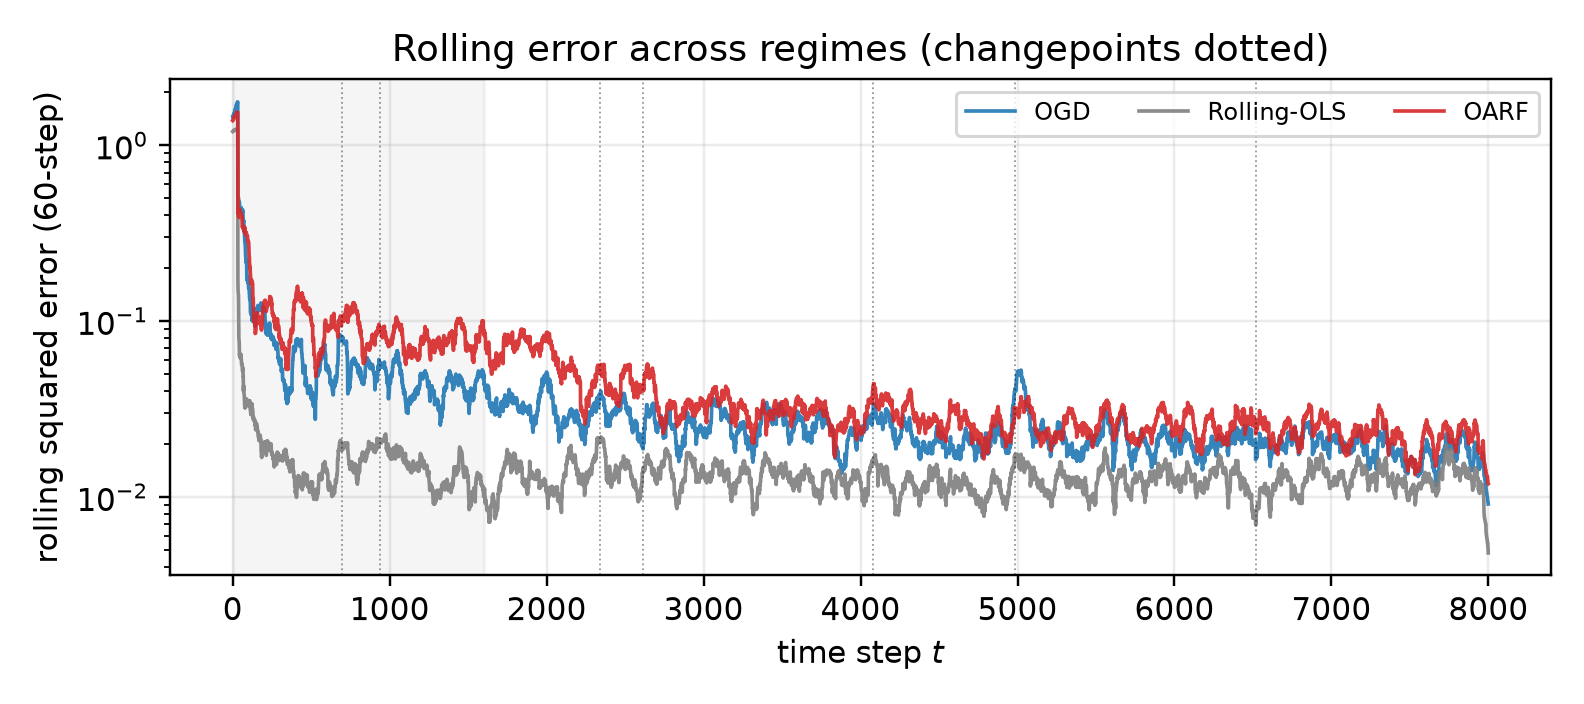
\includegraphics[width=0.86\textwidth]{fig1_rolling_error.png}
\caption{Rolling squared error across regimes on a representative seed (changepoints
dotted, the shaded band is the warm-up window). The reactive baselines spike at every
break; \OARF{} stays comparatively flat.}
\label{fig:rolling}
\end{figure}

\begin{figure}[htbp]
\centering
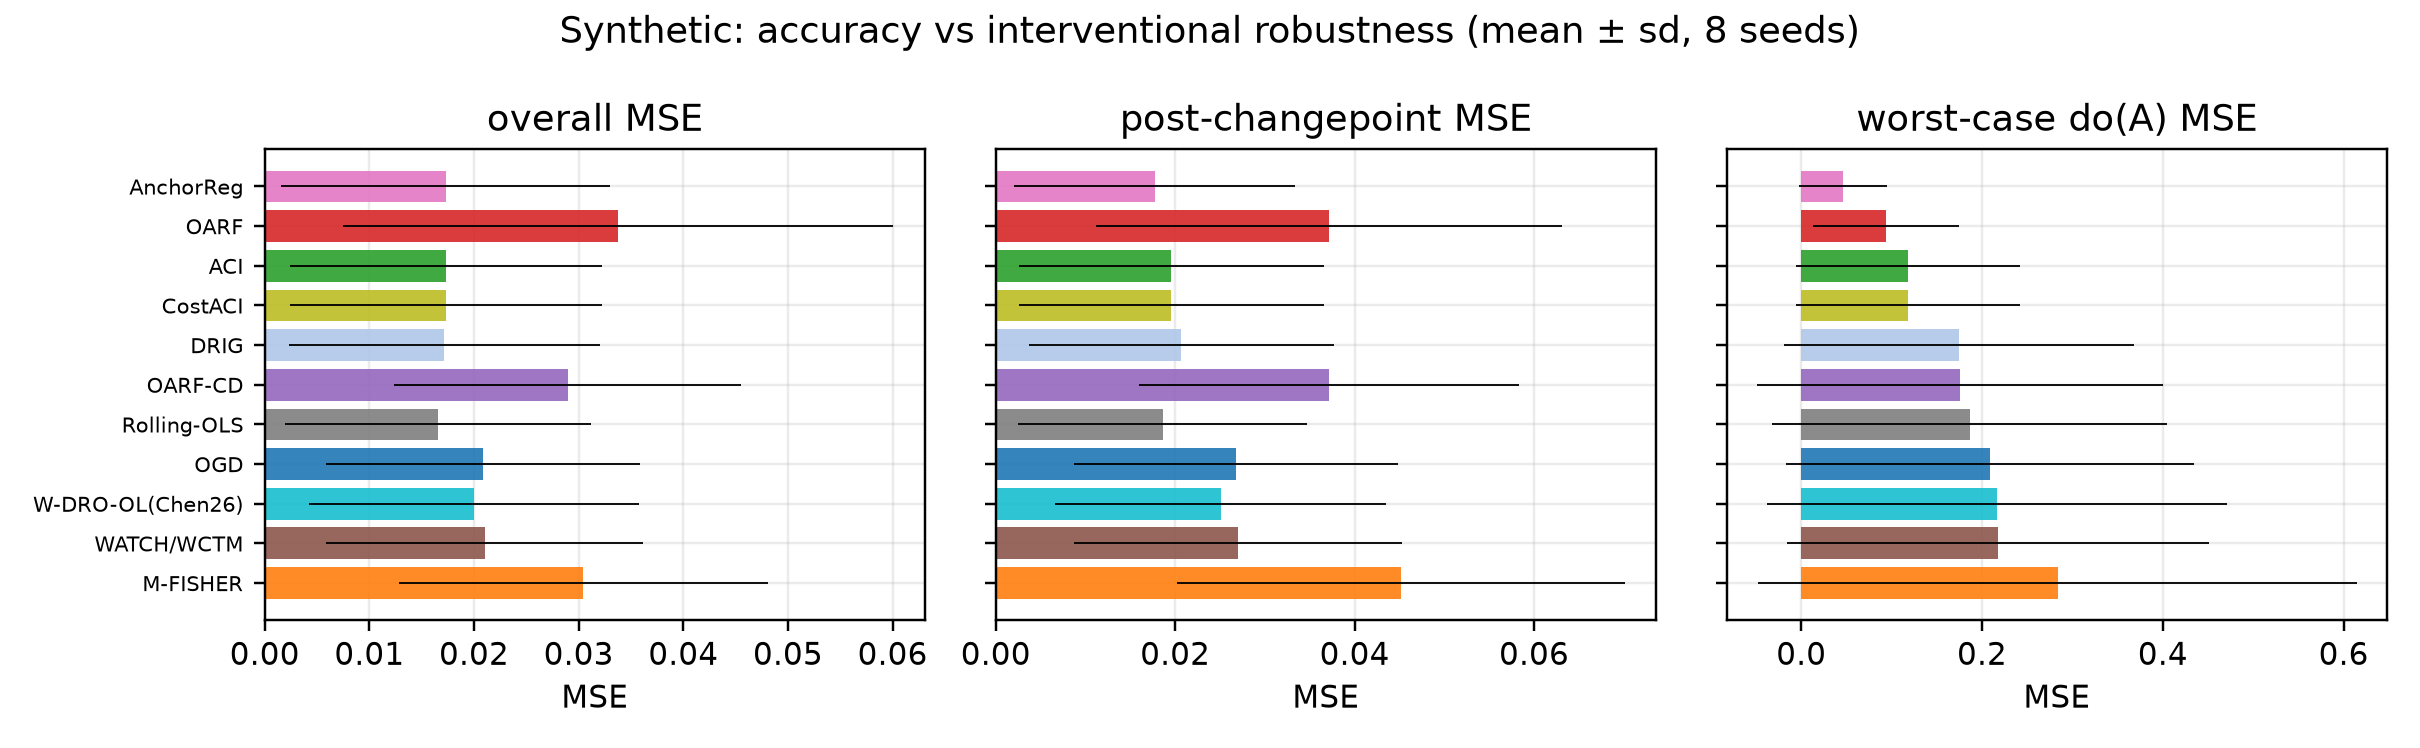
\includegraphics[width=0.92\textwidth]{fig2_bar_metrics.png}
\caption{Overall, post-changepoint and worst-case interventional MSE on the synthetic
benchmark, sorted by interventional robustness. The reactive and batch methods win in
distribution and \OARF{} and the batch oracle win under intervention, so the two panels are
nearly mirror images.}
\label{fig:bars}
\end{figure}

\begin{figure}[htbp]
\begin{subfigure}{0.5\textwidth}\centering
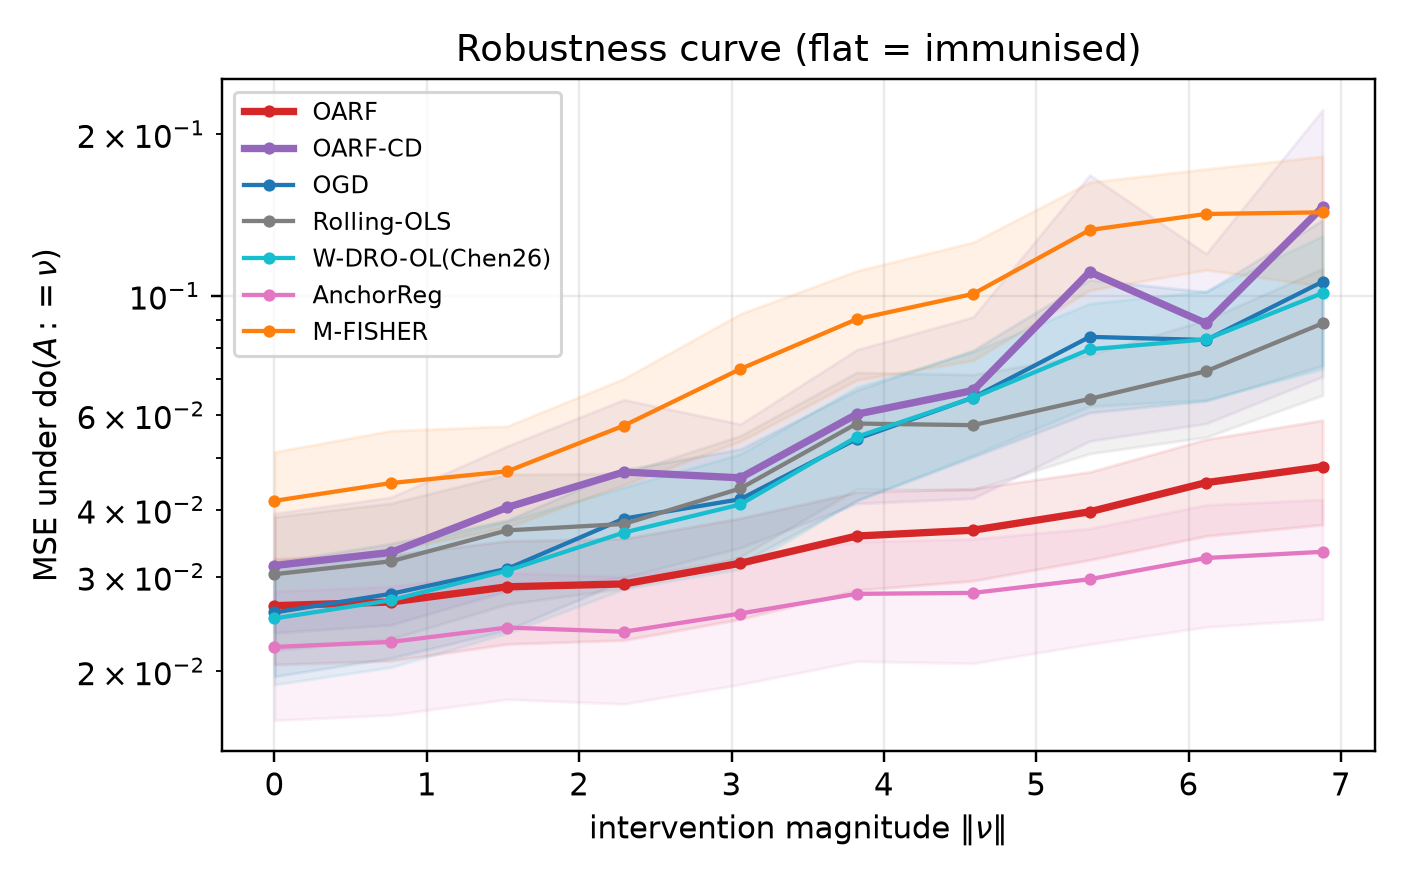
\includegraphics[width=\linewidth]{fig3_robustness_curve.png}
\caption{Robustness curve: MSE against intervention magnitude $\|\nu\|$.}\label{fig:robust}
\end{subfigure}\hfill
\begin{subfigure}{0.5\textwidth}\centering
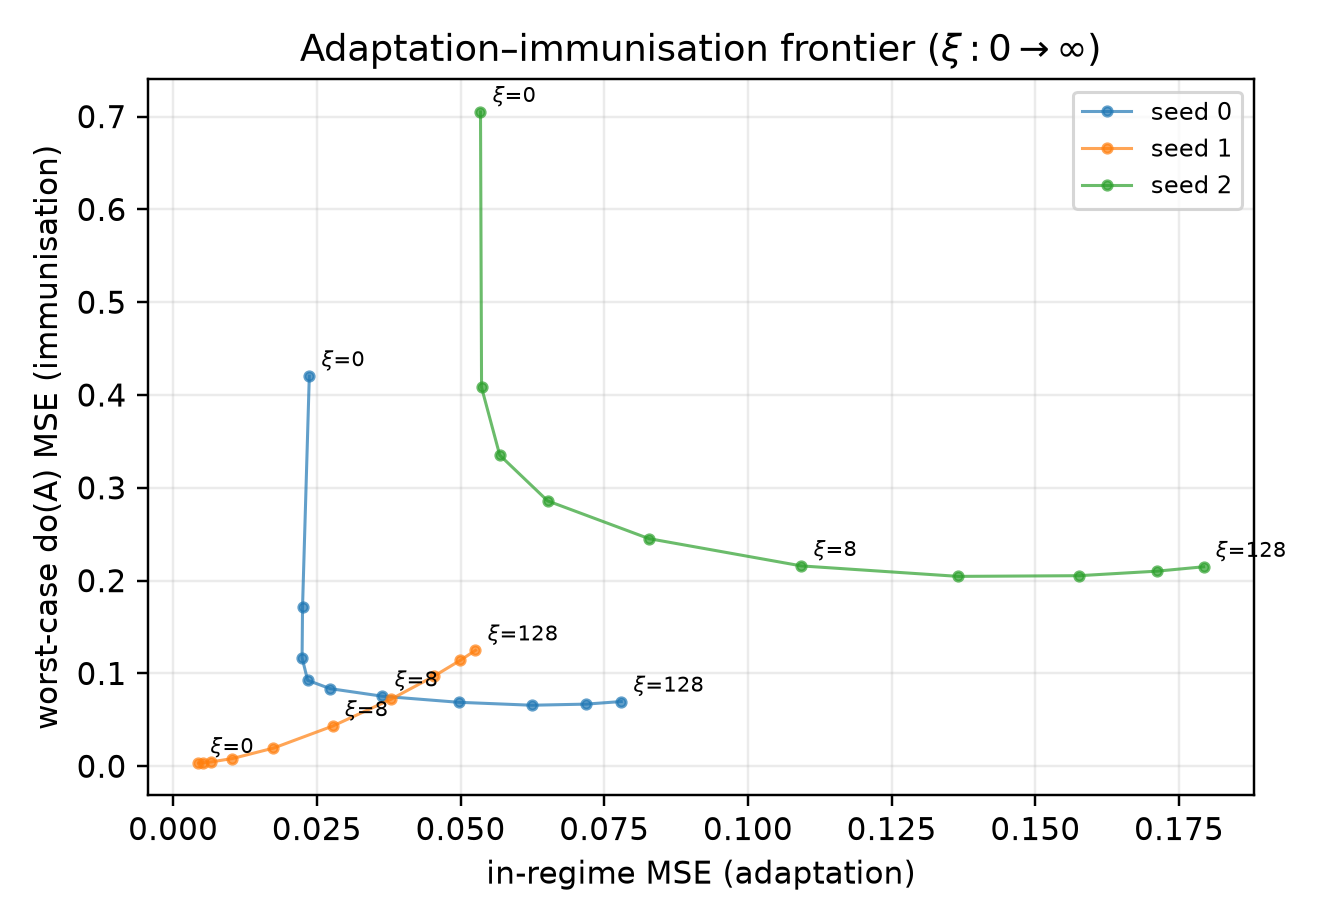
\includegraphics[width=\linewidth]{fig4_pareto.png}
\caption{Adaptation--robustness frontier as $\xi:0\to\infty$.}\label{fig:pareto}
\end{subfigure}
\caption{(a) \OARF{} and the batch oracle remain near-flat as interventions grow, while
reactive and agnostic-robust methods degrade steeply. (b) The penalty $\xi$ moves the
learner continuously from the online-gradient-descent corner to maximal robustness.}
\label{fig:robust-pareto}
\end{figure}

\begin{figure}[htbp]
\centering
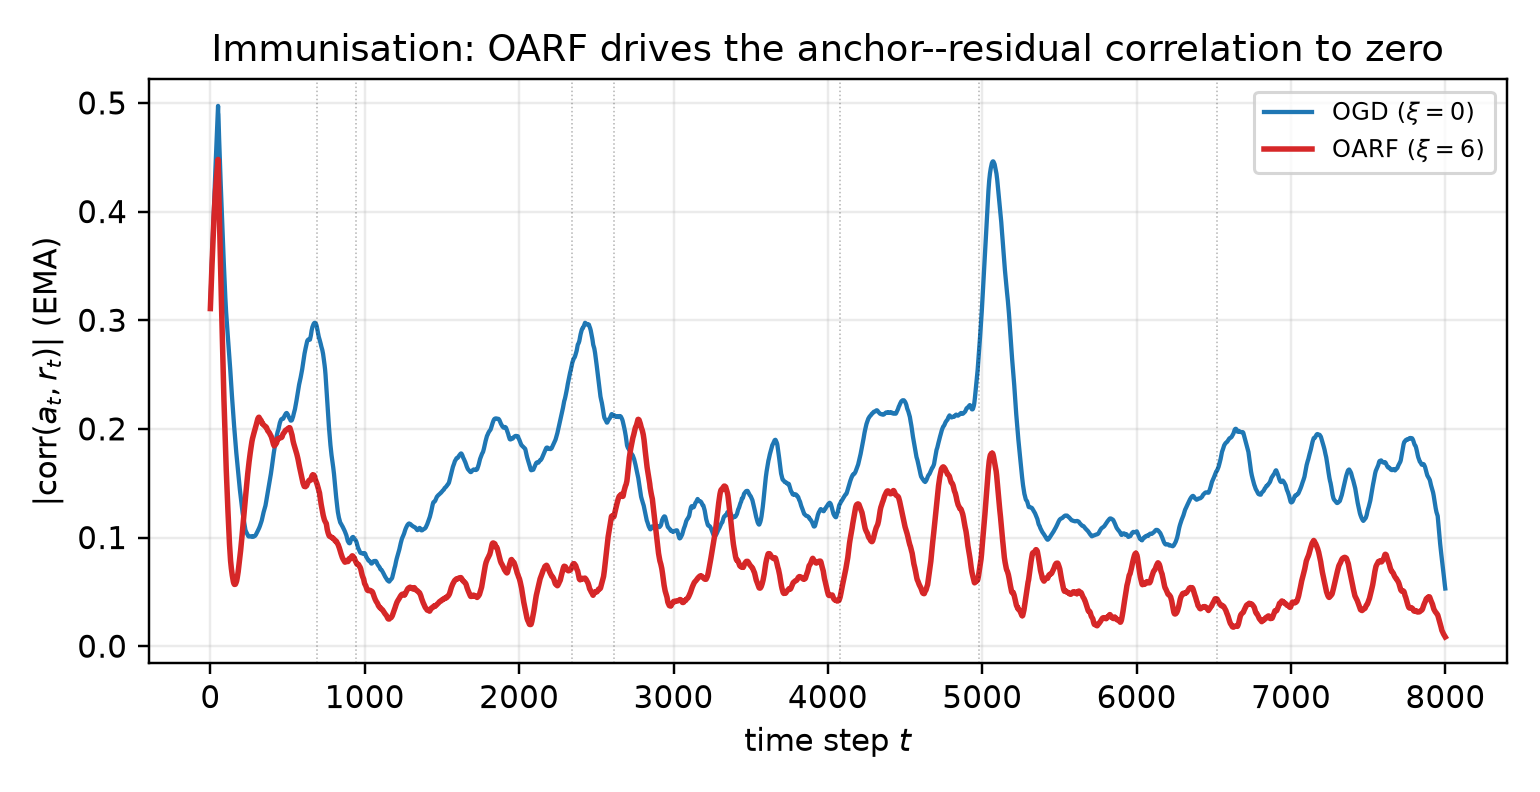
\includegraphics[width=0.78\textwidth]{fig5_immunization.png}
\caption{Anchor--residual correlation. The smoothed correlation
$|\mathrm{corr}(a_t,r_t)|$ is held near zero by \OARF{} ($\xi=6$) but spikes for online
gradient descent ($\xi=0$) at each regime change (dotted).}
\label{fig:immun}
\end{figure}

\paragraph{Learned channel}
When it has to find its own anchor, \OARFCD{} recovers the true subspace on average. Mean
principal-subspace alignment is $0.88\pm0.16$, against a random-subspace baseline of
$0.42$, and individual seeds climb toward $0.99$ as the stream lengthens
(Figure~\ref{fig:channel}). High mean alignment does not give stable robustness, though. A
seed's final alignment is only noisily related to its worst-$\doop(A)$ MSE
(Figure~\ref{fig:scatter}), and the seeds with transiently poor alignment account for the
heavy interventional tail in Table~\ref{tab:syn}. The layer therefore recovers a
nonstationary subspace but does not yet match the reliable interventional robustness of the
fixed channel. It is a proof of concept for removing the analyst-supplied anchor, not yet a
dependable substitute for a known channel, and this tail is the main practical limitation
of the discovery layer.

\begin{figure}[htbp]
\centering
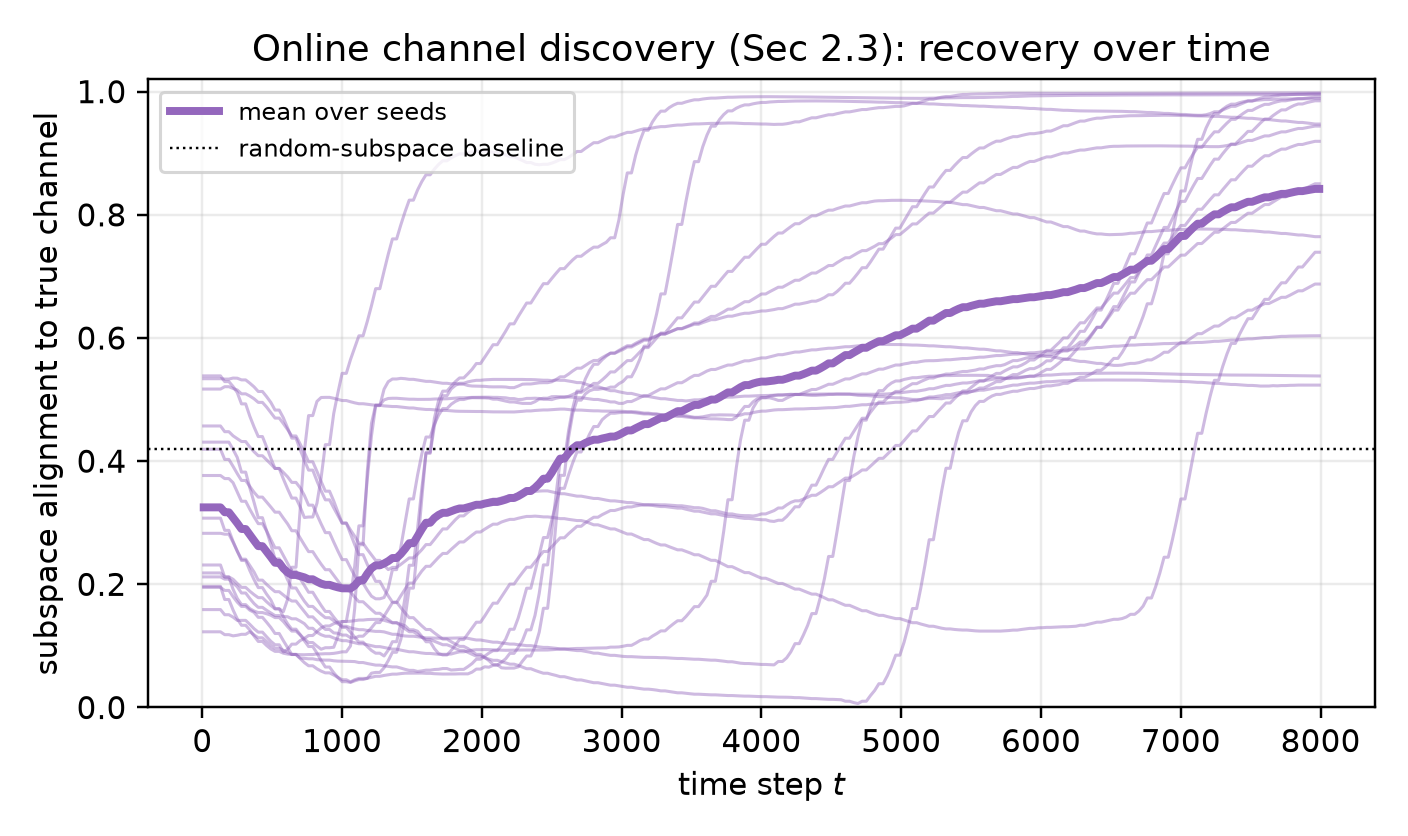
\includegraphics[width=0.72\textwidth]{fig6_learned_channel.png}
\caption{Online channel discovery: alignment of the learned channel $B_t$ to the true
intervention subspace over time. Thin lines are individual seeds, the bold line is their
mean, and the dotted line is the random-subspace baseline.}
\label{fig:channel}
\end{figure}

\begin{figure}[htbp]
\centering
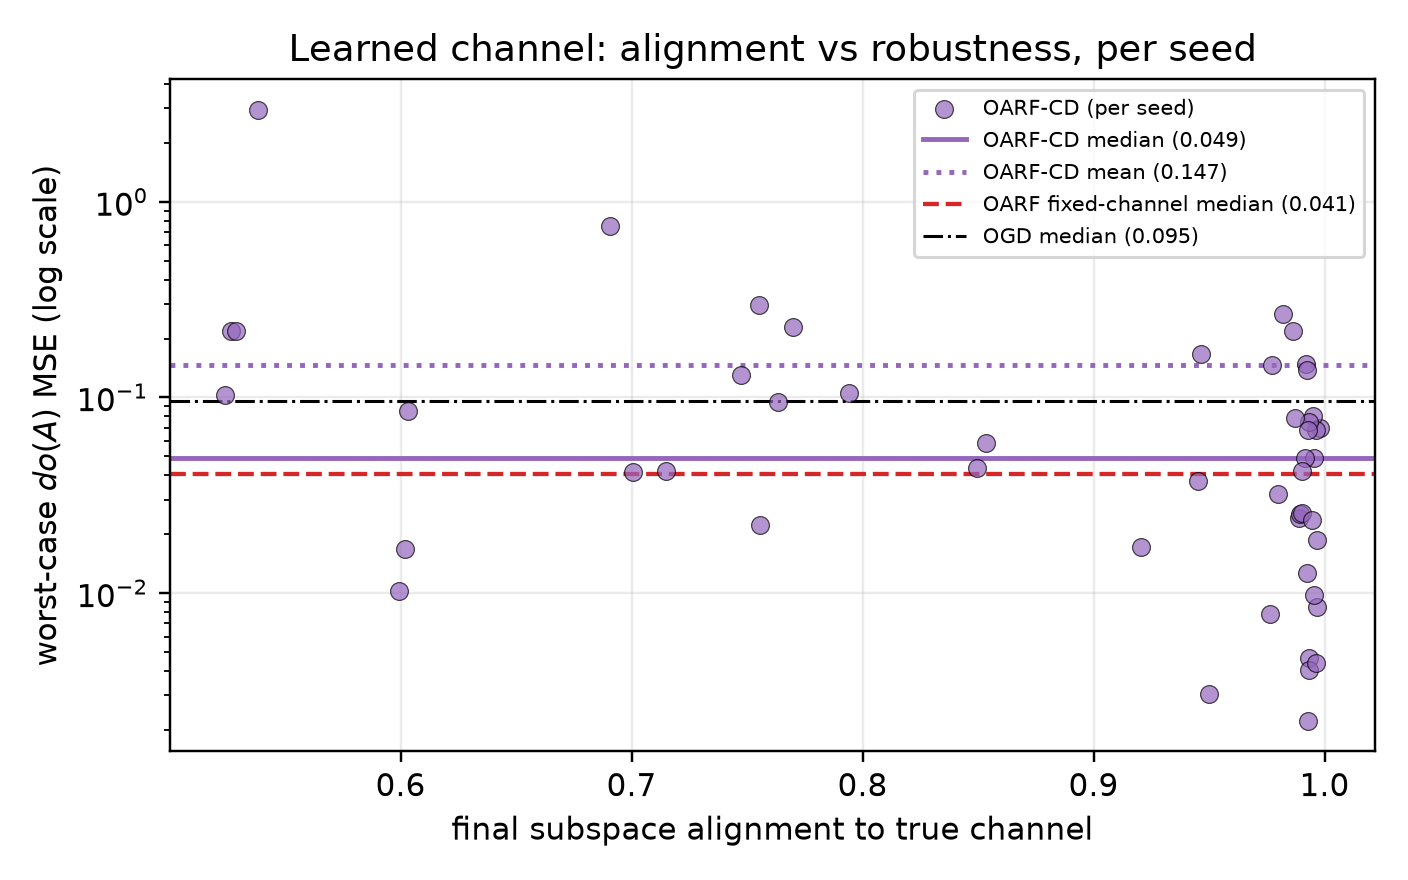
\includegraphics[width=0.74\textwidth]{fig14_alignment_scatter.png}
\caption{Per-seed alignment versus interventional robustness for the learned channel
($50$ seeds). Each point is one seed: the horizontal axis is the final subspace
alignment of \OARFCD{}'s discovered channel and the vertical axis its worst-case
$\doop(A)$ MSE (log scale). High-alignment seeds cluster at low error near the
fixed-channel \OARF{} median (dashed), but a minority of low-alignment seeds incur an
order-of-magnitude higher error. These seeds pull the mean (dotted) far above the median
(solid) and make the learned channel unreliable in the worst case.}
\label{fig:scatter}
\end{figure}

\paragraph{Online reliability diagnostic}
Figure~\ref{fig:scatter} shows that the failures of the discovery layer are a discrete tail
risk. Most seeds recover a well-aligned channel, a minority do not, and those seeds dominate
the mean worst-case error. If they could be flagged while the stream runs, without
consulting the true channel (which a deployment never observes), the layer could decline to
trust its own channel on those streams. Figure~\ref{fig:diagnostic}a tests whether the
eigengap $\kappa$ of Eq.~\eqref{eq:eigengap} can serve as such a flag. Across the $50$
seeds, $\kappa$ correlates with the true subspace alignment, which is otherwise
unobservable, at $r=0.62$, and $13$ of the $16$ seeds whose final alignment falls below
$0.8$ also fall in the bottom quartile of post-warm-up eigengap. Figure~\ref{fig:diagnostic}b
uses this as a gate. When a seed's average post-warm-up $\kappa$ lies in the bottom
quartile (only~$13$ of $50$ seeds), the forecaster reverts to plain OGD; otherwise it
keeps the learned channel. Gating lowers the mean worst-$\doop(A)$ MSE of \OARFCD{} from
$0.147$ (ungated) to $0.113$, a reduction of about a quarter, and closes about two-fifths
of the gap to the $0.059$ attained with the true channel. The gate uses only a statistic the discovery layer already computes. Its threshold, however, is the
$25$th percentile of $\kappa$ across these same $50$ seeds, so in deployment it would
have to be calibrated in advance, for example on simulated streams. The decision uses
the average of $\kappa$ over the second half of each stream, so the gate makes one choice per stream. It also discards a misspecified channel
instead of correcting it; like Davis--Kahan, a large gap certifies a well-identified
subspace but says nothing about whether that subspace is exogenous.

\begin{figure}[htbp]
\centering
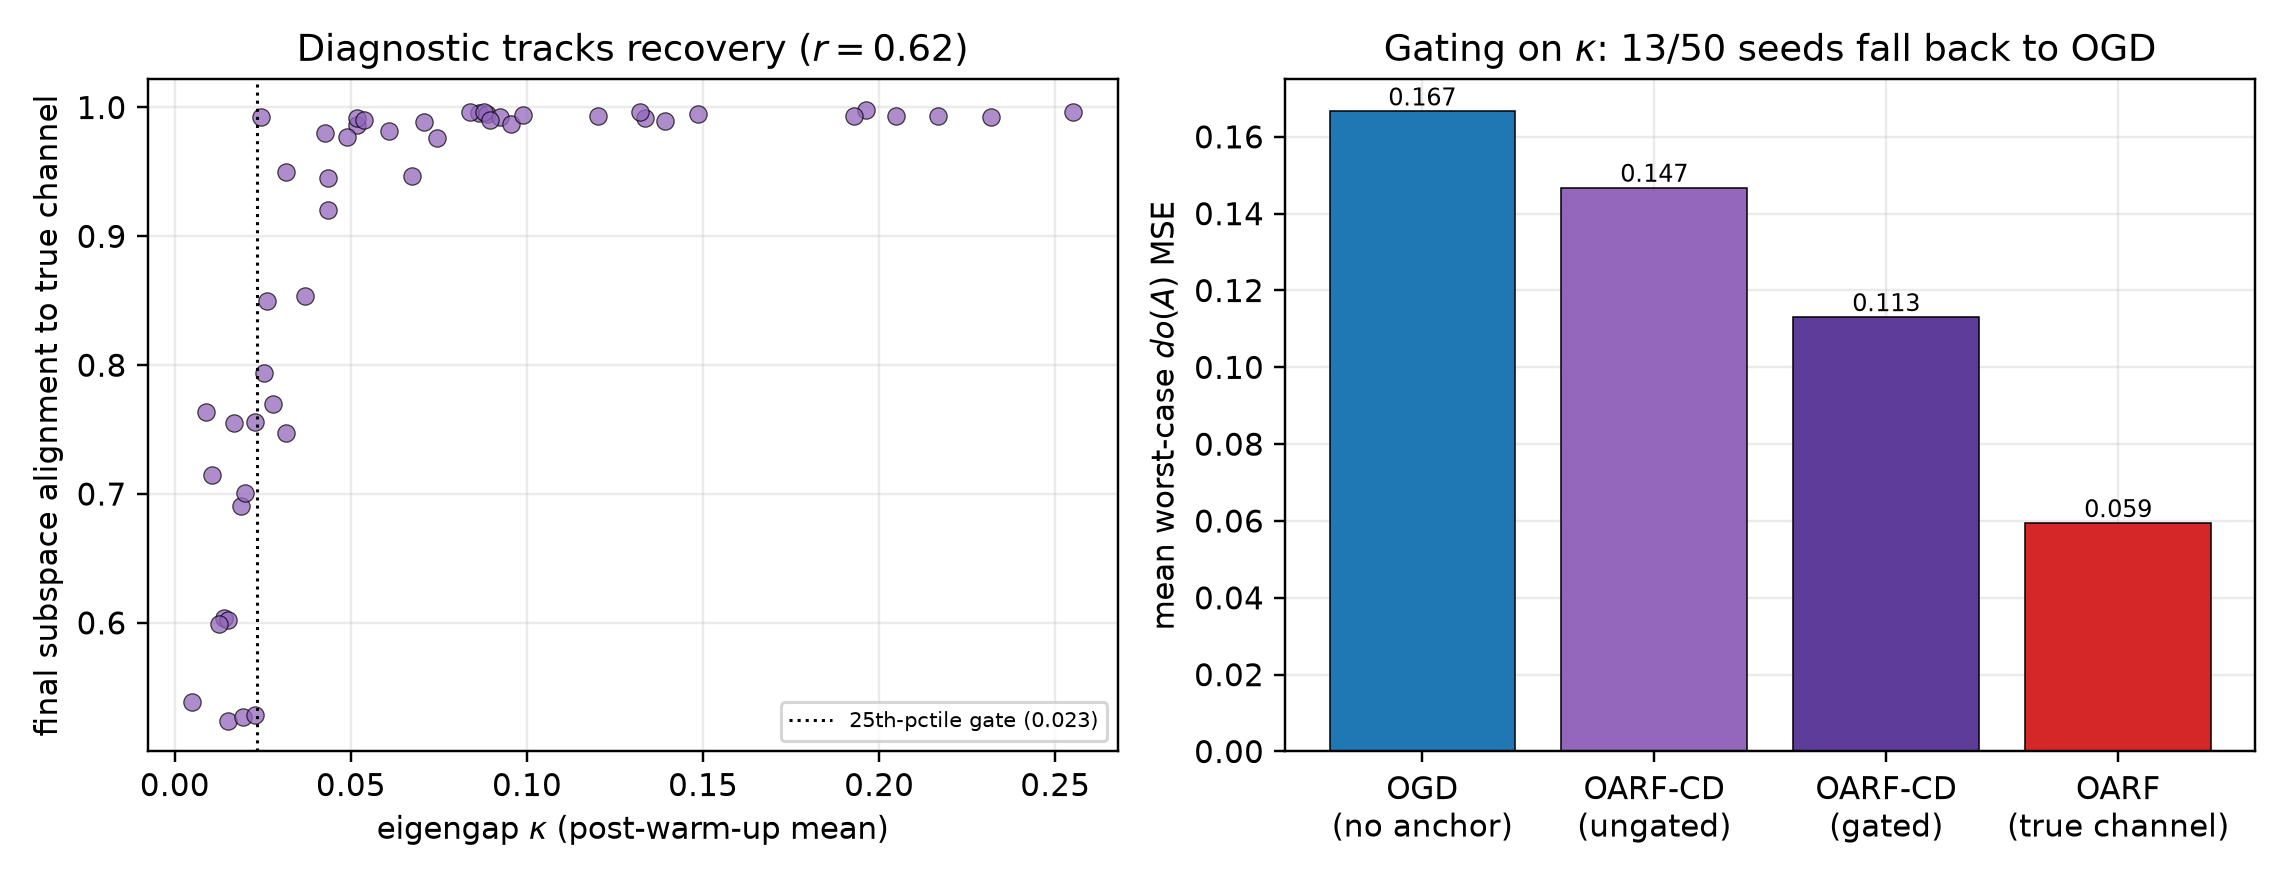
\includegraphics[width=0.98\textwidth]{fig16_eigengap_diagnostic.png}
\caption{Eigengap diagnostic. (a) Per-seed post-warm-up eigengap
$\kappa$ vs.\ true subspace alignment ($r=0.62$); the dotted line is the
$25$th-percentile gate. (b) Mean worst-case $\doop(A)$ MSE for OGD, ungated
\OARFCD{}, \OARFCD{} gated on $\kappa$, and fixed-channel \OARF{} with the true
channel. Gating reduces the ungated learned channel's mean worst-case error by about a
quarter without using the ground truth.}
\label{fig:diagnostic}
\end{figure}

\paragraph{Ablations}
Table~\ref{tab:abl} and Figure~\ref{fig:abl} remove one component at a time. Most of the
interventional robustness comes from the anchor channel. With the true channel the
worst-case interventional error is $0.080$. With a random channel it rises to $0.377$,
which is worse than using no anchor penalty at all (OGD, $0.226$). A wrong channel
therefore does active harm, so identifying the right channel is the main problem; the
stress tests below measure the same effect continuously. The learned channel ($0.303$, alignment $0.84$) is worse than OGD on average in this experiment and, as Table~\ref{tab:syn}
shows, unstable across seeds. AdaGrad matters for both accuracy and robustness: a tuned
fixed step raises in-regime MSE from $0.035$ to $0.095$ and worst-$\doop(A)$ from $0.080$
to $0.145$. EMA centring improves in-regime accuracy ($0.035$ vs.\ $0.043$) with
essentially unchanged robustness, which is consistent with separating the regime mean from
the covariance the penalty uses. For the discovered dimension, worst-$\doop(A)$ MSE and
alignment both improve gradually as $q$ rises from $1$ to $4$ ($0.329\!\to\!0.261$,
alignment $0.79\!\to\!0.90$), because a larger learned subspace still contains the true
two-dimensional channel. Under-specifying the dimension ($q=1$) does more damage, because
the smaller subspace cannot contain it. Results are broadly insensitive to the EMA decay
$\beta$ over $[0.90,0.995]$.

\begin{table}[htbp]
\centering
\caption{Component ablations on the synthetic benchmark (mean over 16 seeds, $\xi=6$
unless noted). The channel carries most of the interventional robustness, and a wrong
channel is worse than none.}
\label{tab:abl}
\small
\begin{tabular}{lcc}
\toprule
Variant & in-regime MSE & worst-$\doop(A)$ MSE\\
\midrule
\OARF{} (full, true channel) & $0.035$ & $\mathbf{0.080}$\\
\quad $-$ EMA centring        & $0.043$ & $0.081$\\
\quad $-$ AdaGrad (fixed step) & $0.095$ & $0.145$\\
\quad random channel          & $0.032$ & $0.377$\\
\quad $\xi=0$ (OGD)           & $0.027$ & $0.226$\\
\midrule
learned channel (\OARFCD{}, alignment $0.84$) & $0.033$ & $0.303$\\
\bottomrule
\end{tabular}
\end{table}

\begin{figure}[htbp]
\centering
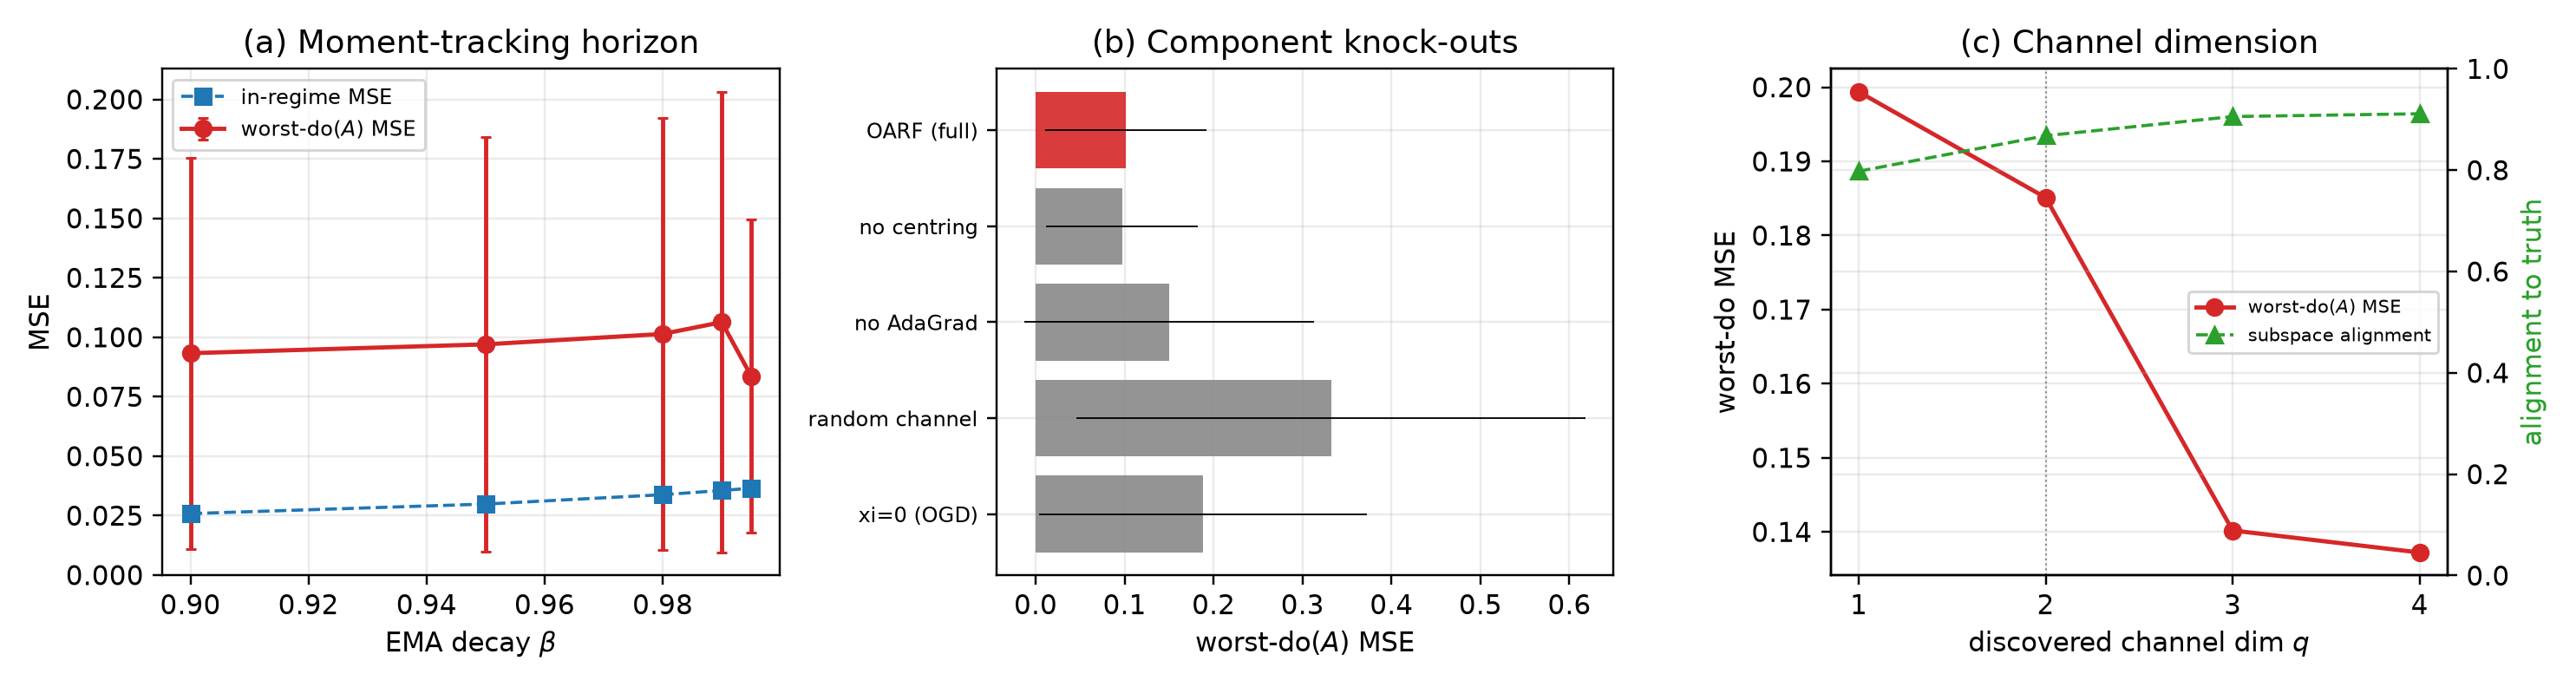
\includegraphics[width=0.99\textwidth]{fig11_ablations.png}
\caption{Ablations. (a) Sensitivity to the EMA decay $\beta$. (b) Component knock-outs by
worst-case interventional MSE: the channel and the adaptive step matter most, and a
random channel is worse than none. (c) Discovered-channel dimension: robustness and alignment both improve slightly with $q$ (true $q=2$ dotted), but worst-case error stays above OGD at every $q$.}
\label{fig:abl}
\end{figure}
\paragraph{Stress tests}
The synthetic benchmark favours \OARF{} by construction, because the anchor is clean and
fully observed. In practice it may be neither, so we stress the fixed-channel method
along two axes that break these conditions (Figure~\ref{fig:stress}; the synthetic SCM
is otherwise unchanged, 8 seeds). First, we add noise of growing scale to the observed
context before any method sees it. Worst-$\doop(A)$ MSE rises monotonically with the
noise scale, and \OARF{} crosses the no-anchor OGD baseline at roughly one standard
deviation of observation noise ($0.18$ vs.\ OGD $0.19$). Beyond that point a noisy
anchor is no better than no anchor, and the learned channel degrades sooner. Second, we
rotate the supplied channel away from the truth by an angle $\theta$ (subspace
alignment $\cos\theta$). \OARF{} beats OGD while the alignment exceeds about $0.6$
(roughly $\theta\le 50^\circ$). With a more misaligned channel it is worse than OGD,
reaching $0.36$ against OGD's $0.19$ when the channel is orthogonal; the random-channel
row of Table~\ref{tab:abl} reflects the same mechanism. \OARF{} should therefore be
deployed only when the analyst has reason to believe the anchor is informative, that
is, with alignment well above $0.6$ and noise below order one. A weak or guessed channel can make forecasts worse than using no anchor.

\begin{figure}[htbp]
\centering
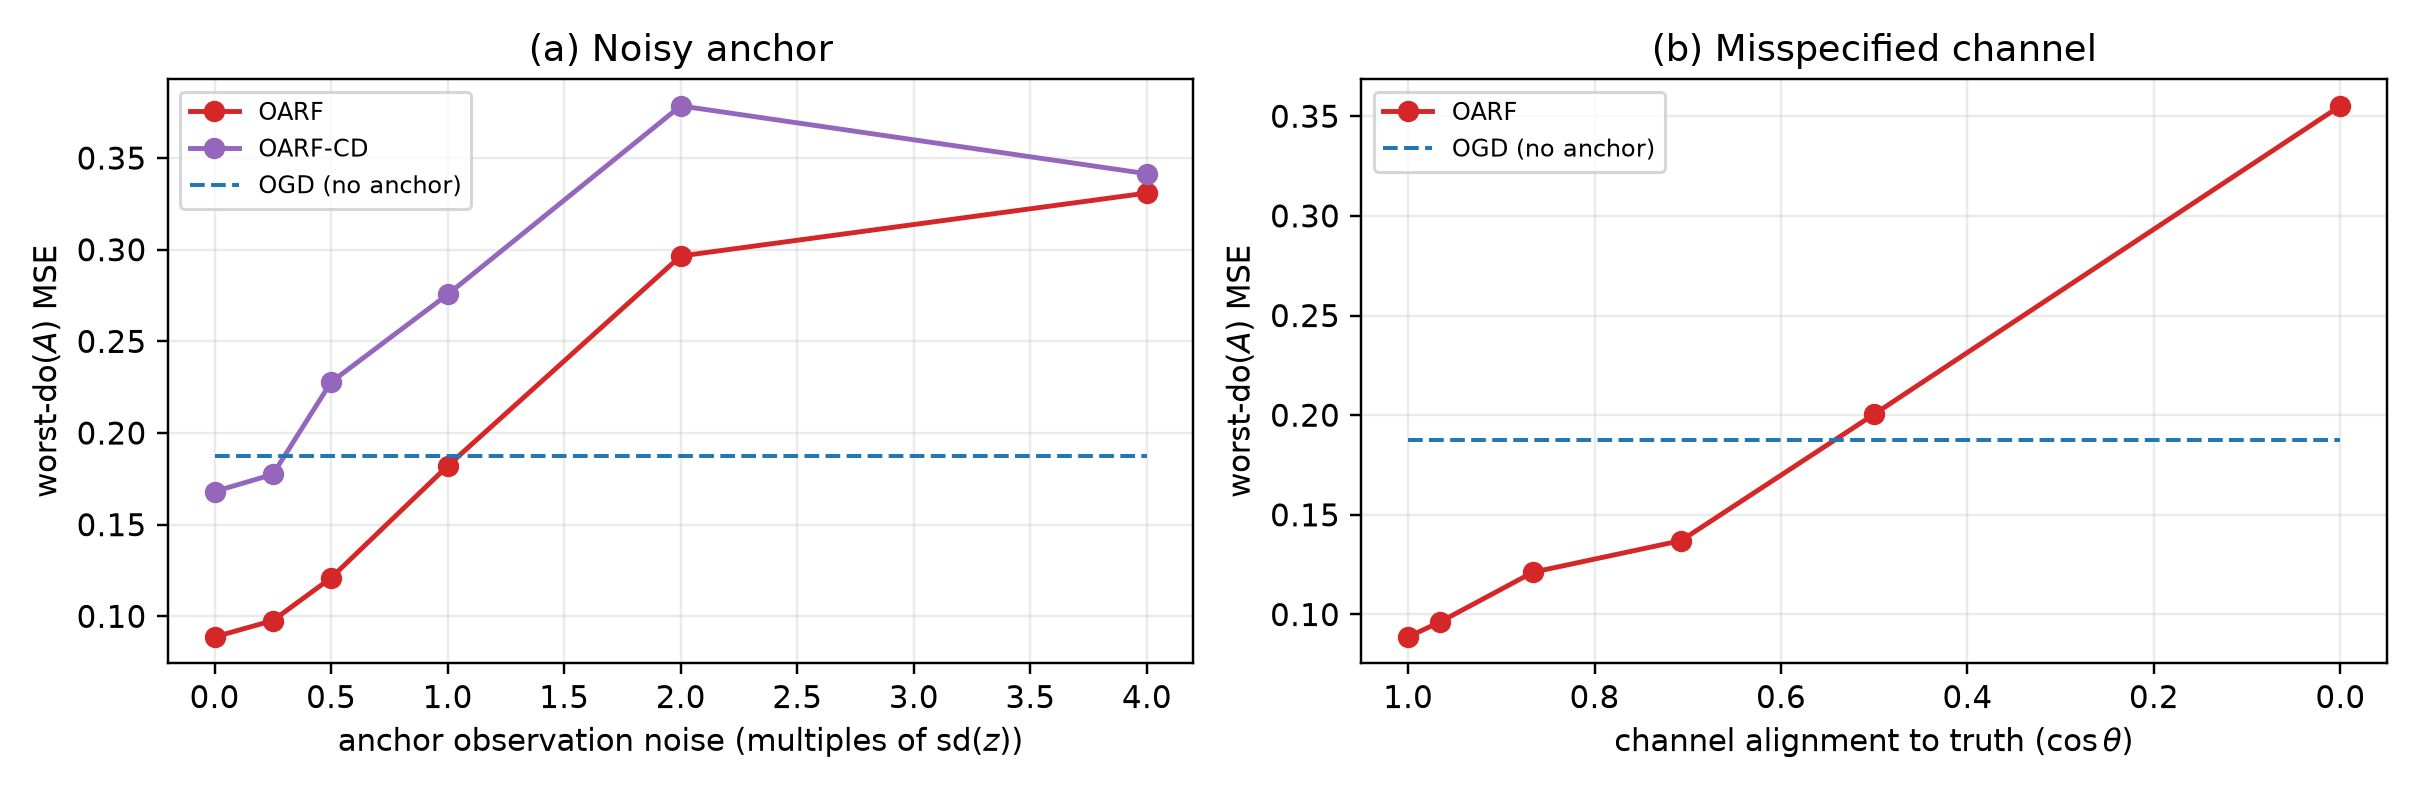
\includegraphics[width=0.97\textwidth]{fig12_stress.png}
\caption{Stress tests of the fixed-channel method (worst-$\doop(A)$ MSE; OGD baseline
dashed). (a) Increasing anchor observation noise: \OARF{} crosses the no-anchor baseline
near one standard deviation of noise. (b) Rotating the channel away from the truth:
anchoring helps while alignment $\cos\theta\gtrsim 0.6$ and hurts beyond that
point.}
\label{fig:stress}
\end{figure}

\paragraph{Assumption-violation scenarios}
The stress tests vary the quality of the anchor. We also change the SCM structure so as
to break the assumptions behind Proposition~\ref{prop:equiv} one at a time
(Table~\ref{tab:scen}, median worst-$\doop(A)$ MSE over 8 seeds). \OARF{} keeps its
advantage over OGD in three of these scenarios: when the intervention also shifts the
parents (\textsc{parents}), because the invariant predictor remains valid; when a second
regime driver is unobserved (\textsc{unobserved}), because robustifying the observed
part still helps; and when the observed anchor is a noisy proxy for the true latent
driver (\textsc{proxy}). The method therefore degrades gradually under these
violations. It fails in two cases. When the regime shifts the target's own
parent-coefficient (\textsc{mechanism}), no fixed predictor is robust and both methods
collapse ($\ge\!1.0$). When regimes shift the variance instead of the mean
(\textsc{variance}), the mean-shift equivalence does not apply and \OARF{} is worse than
OGD. The theory covers neither case, and we regard both as limitations of the method.

\begin{table}[htbp]
\centering
\caption{Assumption-violation scenarios (median worst-$\doop(A)$ MSE over 8 seeds;
lower is better). \OARF{} uses the true observed channel. It fails under a shifting
target mechanism and when regimes shift the variance instead of the mean.}
\label{tab:scen}
\small
\begin{tabular}{lcccl}
\toprule
Scenario & \OARF{} & \OARFCD{} & OGD & assumption broken\\
\midrule
clean (ideal)      & $0.021$ & $0.033$ & $0.051$ & none (reference)\\
parents shifted    & $0.018$ & $0.016$ & $0.047$ & none (still anchor-mediated)\\
unobserved driver  & $0.024$ & $0.040$ & $0.048$ & channel incompletely observed\\
noisy proxy anchor & $0.044$ & $0.058$ & $0.065$ & anchor predictive, not causal\\
\midrule
mechanism shift    & $1.299$ & $1.238$ & $1.020$ & target mechanism non-invariant\\
variance shift     & $0.046$ & $0.040$ & $0.025$ & regimes shift variance, not mean\\
\bottomrule
\end{tabular}
\end{table}

\paragraph{Comparison of anchor selectors}
Automatic anchor selection is the most fragile part of the method, so we compare the
block-mean rule of OARF-CD with alternative selectors under a strict pre-deployment
budget: the channel is estimated on the warm-up block only, with no look-ahead
(Table~\ref{tab:sel}). The alternatives are a supervised residual--context-coupling
selector, stationary PCA of the context, and a random channel. Each is scored by its
alignment to the truth and by the worst-$\doop(A)$ MSE of the resulting fixed-channel
method. The block-mean rule does about as well as the supervised selector and much better than stationary PCA. From a short warm-up, though, neither is clearly better than a random channel: their worst-$\doop(A)$ MSEs are $0.101$ and $0.093$ against $0.115$ for a random channel and $0.070$ for the true one, and their alignments ($0.42$ and $0.37$) are no higher than the random channel's ($0.43$). High alignment is reached only by learning over the full stream (\OARFCD{}, alignment $0.84$ in Table~\ref{tab:abl}), and even then the estimate is unstable.
Reliable online anchor discovery from limited data thus remains an open problem.
Practitioners should supply a candidate anchor and validate it with the procedure
below instead of relying on automatic discovery alone.

\begin{table}[htbp]
\centering
\caption{Anchor selectors estimated on the warm-up block only (8 seeds; alignment to
the true channel, and worst-$\doop(A)$ MSE of the resulting fixed-channel \OARF{};
lower MSE / higher alignment better).}
\label{tab:sel}
\small
\begin{tabular}{lcc}
\toprule
Selector & subspace alignment & worst-$\doop(A)$ MSE (median)\\
\midrule
true channel (reference)             & $1.00$ & $0.070$\\
block-mean (OARF-CD rule)            & $0.42$ & $0.101$\\
supervised residual--context coupling & $0.37$ & $0.093$\\
stationary PCA of context            & $0.31$ & $0.236$\\
random channel                       & $0.43$ & $0.115$\\
\bottomrule
\end{tabular}
\end{table}

\paragraph{Diagnostics and an anchor-selection procedure}
The stress tests, scenarios and selector comparison lead to a practical procedure.
Before trusting \OARF{}, and \OARFCD{} in particular, a practitioner should: (1) propose
candidate anchors from domain knowledge (for energy, the macro-uncertainty indices);
(2) estimate the anchor--residual correlation of a plain online learner and check that
it is non-trivial and stable over the warm-up; (3) run a warm-up stress test,
perturbing the anchor artificially as in Figure~\ref{fig:stress}, and confirm that
anchoring improves validation worst-regime loss without an unacceptable
in-distribution cost; (4) for \OARFCD{}, monitor whether the learned subspace
stabilises and aligns with interpretable drivers, and fall back to a fixed anchor or to
$\xi=0$ (plain OGD) if it does not. The checklist below summarises the resulting decision rule.

\begin{center}
\fbox{\begin{minipage}{0.92\linewidth}
\small
\textbf{Pre-deployment checklist for \OARF{}.}\\[2pt]
Use fixed-channel \OARF{} when the anchor has a domain justification; the
anchor--residual correlation is non-trivial and stable over the warm-up; a warm-up
stress test shows anchoring improves validation worst-regime loss; and random-channel
and noisy-anchor diagnostics do not match or beat the chosen anchor.\\[3pt]
Do not use \OARF{} (fall back to OGD/ACI) when the learned or chosen channel is
unstable across the warm-up; validation performance is no better than plain OGD; the
regime shifts appear as variance shifts or direct mechanism shifts instead of
anchor-mediated mean shifts; or the anchor noise is high. Treat \OARFCD{} as a
diagnostic only, and do not deploy its channel unless it passes these checks.
\end{minipage}}
\end{center}

\paragraph{Real data}
The energy panel (Table~\ref{tab:real}) checks whether the mechanism carries over to real series. On both targets the $10\%$ Model Confidence Set retains $10$ of the $11$ methods and excludes only M-FISHER ($p=0.008$ on Brent). Every retained method has an MCS $p$-value of $1.00$ except the Expected-Shortfall combiner ($p=0.22$ on Brent), so the differences among retained methods in Table~\ref{tab:real} are not significant, and \OARF{} is competitive with the strongest baselines without being better than them. The most likely reason is that real energy
variance has weaker, noisier driver--residual coupling than the controlled SCM. The
stress tests above predict that the anchor advantage shrinks toward zero in that
setting, which is what we observe. The conformal head's
coverage is near nominal ($0.90$). A decision-economic volatility-timing check in the appendix finds that over this sample the risk-targeting Sharpe ratios are low and
statistically indistinguishable across methods.
An event study around the COVID-19 crash and the 2022 energy shock
(Appendix~\ref{app:events}) gives the same picture for dated episodes. \OARF{} holds
the anchor--residual correlation below OGD's in every window, but it has a loss
advantage in only one of four event/commodity windows. The anchor mechanism is active,
yet too weakly coupled to give a dependable gain.

\begin{table}[htbp]
\centering
\caption{Real energy log daily-variance-proxy combination, 2010--2026 evaluation window
(lower is better). Ten of the eleven methods lie within the 10\% Model Confidence Set
(MCS $p=1.00$ for all but the Expected-Shortfall combiner, $p=0.22$ on Brent); only M-FISHER is excluded ($p=0.008$ on Brent). The differences
among the retained methods are not statistically significant and are reported
descriptively.}
\label{tab:real}
\small
\begin{tabular}{lcccc|cccc}
\toprule
& \multicolumn{4}{c|}{\textbf{Brent (DCOILBRENTEU)}}
& \multicolumn{4}{c}{\textbf{Henry Hub (DHHNGSP)}}\\
Method & MSE & w-reg & post-cp & cov & MSE & w-reg & post-cp & cov\\
\midrule
\textbf{\OARF{}}   & $0.2225$ & $0.2313$ & $0.2384$ & --     & $0.2870$ & $0.3928$ & $0.2670$ & --\\
\textbf{\OARFCD{}} & $0.2225$ & $0.2292$ & $0.2433$ & --     & $0.2857$ & $0.3850$ & $0.2627$ & --\\
OGD                & $0.2243$ & $0.2334$ & $0.2412$ & --     & $0.2860$ & $0.3888$ & $0.2655$ & --\\
Rolling-OLS        & $0.2203$ & $0.2230$ & $0.2358$ & --     & $0.2882$ & $0.3916$ & $0.2623$ & --\\
ACI                & $0.2180$ & $0.2221$ & $0.2399$ & $0.900$& $0.2808$ & $0.3833$ & $0.2426$ & $0.904$\\
M-FISHER (2025)    & $0.2680$ & $0.2691$ & $0.3307$ & --     & $0.3532$ & $0.4428$ & $0.3442$ & --\\
DR-Combo (Wang 2026)& $0.2304$ & $0.2325$ & $0.2507$ & --    & $0.2891$ & $0.3958$ & $0.2432$ & --\\
FC-DRO (Liu 2026)  & $0.2318$ & $0.2346$ & $0.2571$ & --     & $0.2872$ & $0.3916$ & $0.2436$ & --\\
FC-DRO-ES (Liu 2026)& $0.2387$& $0.2440$ & $0.2713$ & --     & $0.3056$ & $0.4086$ & $0.2689$ & --\\
W-DRO-OL (Chen 2026)& $0.2243$& $0.2334$ & $0.2406$ & --     & $0.2859$ & $0.3890$ & $0.2633$ & --\\
AnchorReg          & $0.2183$ & $0.2195$ & $0.2345$ & --     & $0.2907$ & $0.3942$ & $0.2716$ & --\\
\bottomrule
\end{tabular}
\end{table}

\begin{figure}[htbp]
\centering
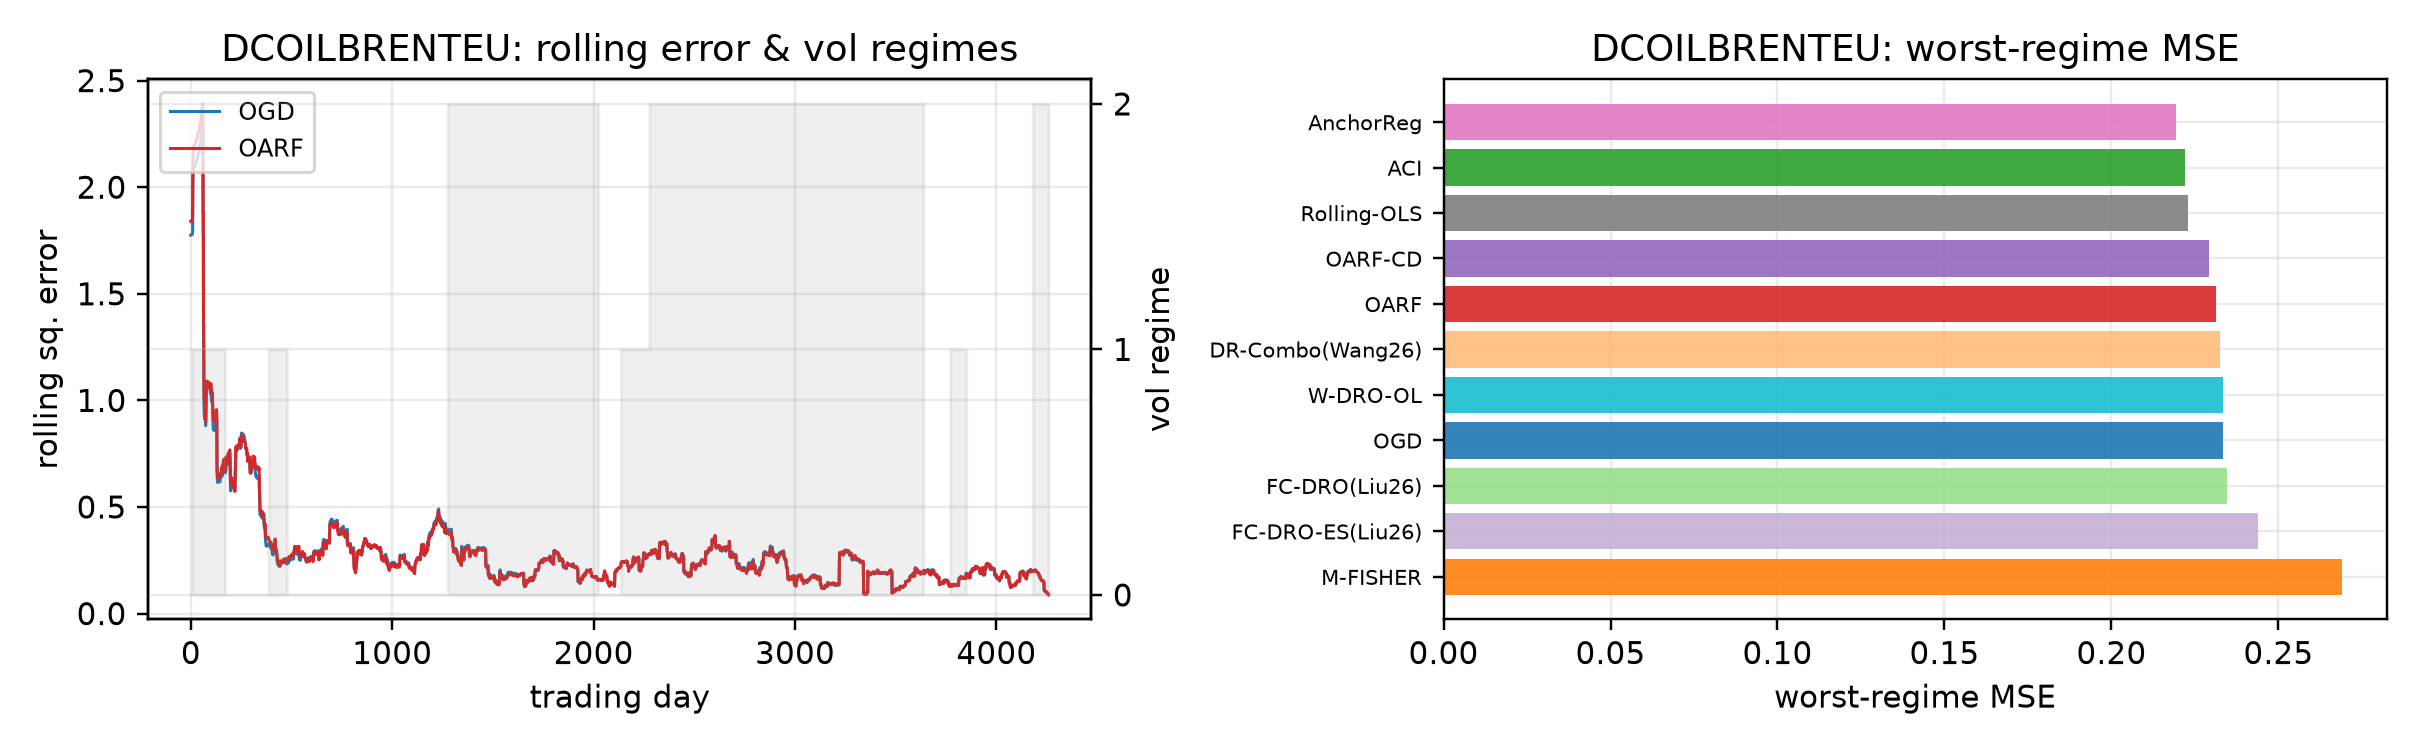
\includegraphics[width=0.97\textwidth]{fig9_real_DCOILBRENTEU.png}
\caption{Brent: rolling squared error with the volatility-regime overlay (left) and
worst-regime MSE by method (right).}
\label{fig:real}
\end{figure}

\begin{figure}[htbp]
\centering
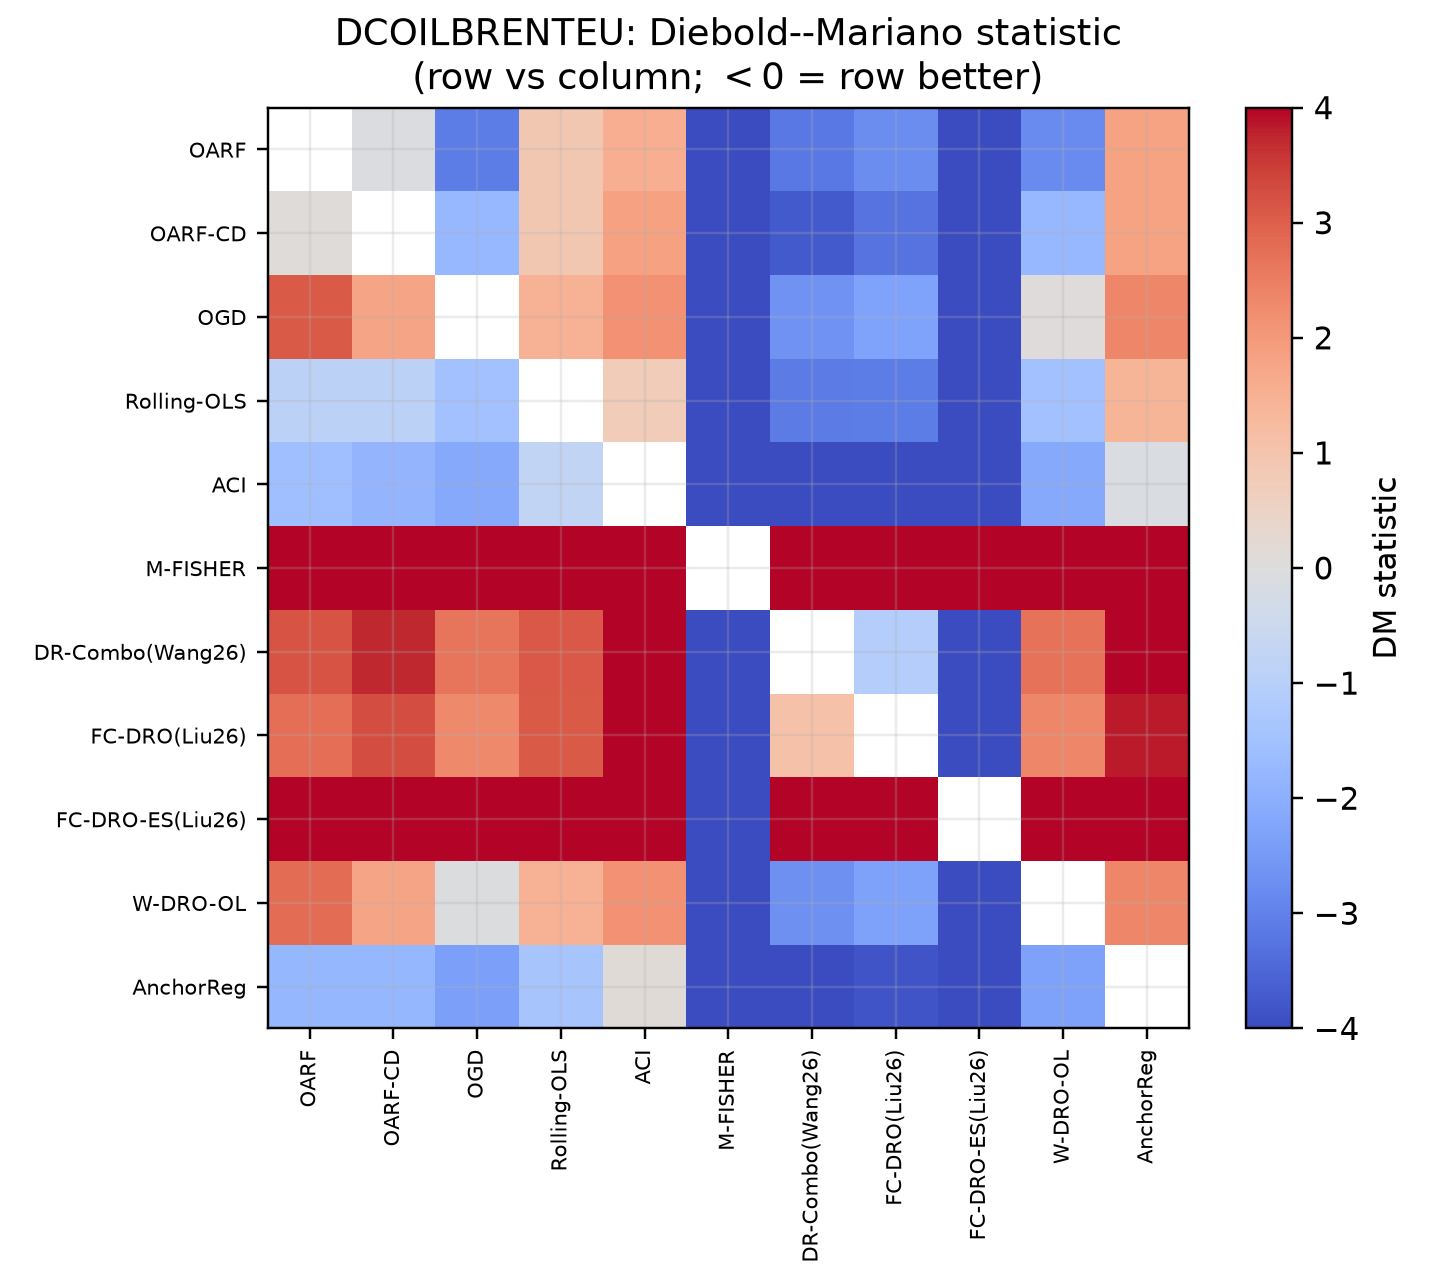
\includegraphics[width=0.6\textwidth]{fig13_dm_DCOILBRENTEU.png}
\caption{Brent: pairwise Diebold--Mariano statistics (negative = row more accurate
than column). Most pairs are small in magnitude, consistent with the Model Confidence Set retaining ten of the eleven methods.}
\label{fig:real-dm}
\end{figure}

\paragraph{Significance}
The two Model Confidence Set analyses show what the evidence supports. On the synthetic
benchmark, the set computed on in-distribution loss (over 16 seeds) retains the
batch and conformal methods (Rolling-OLS in all 16 seeds, DRIG in 15, the conformal
heads in 11) and excludes fixed-channel \OARF{} (retained in 0 seeds) and \OARFCD{}
(1 seed), because \OARF{} gives up some in-distribution accuracy
in exchange for interventional robustness, which in-distribution loss does not reward;
the relevant evaluation for \OARF{} is the held-out intervention grid. On the real
targets the MCS retains $10$ of $11$ methods on each commodity (only the weakest is
excluded), so no method significantly out-predicts the others on average, and the
real-data differences are descriptive, as noted above. The Diebold--Mariano statistics
agree: they are pronounced on the synthetic benchmark (Figure~\ref{fig:dm}) and mostly
small on the real targets (Figure~\ref{fig:real-dm}).

\begin{figure}[htbp]
\centering
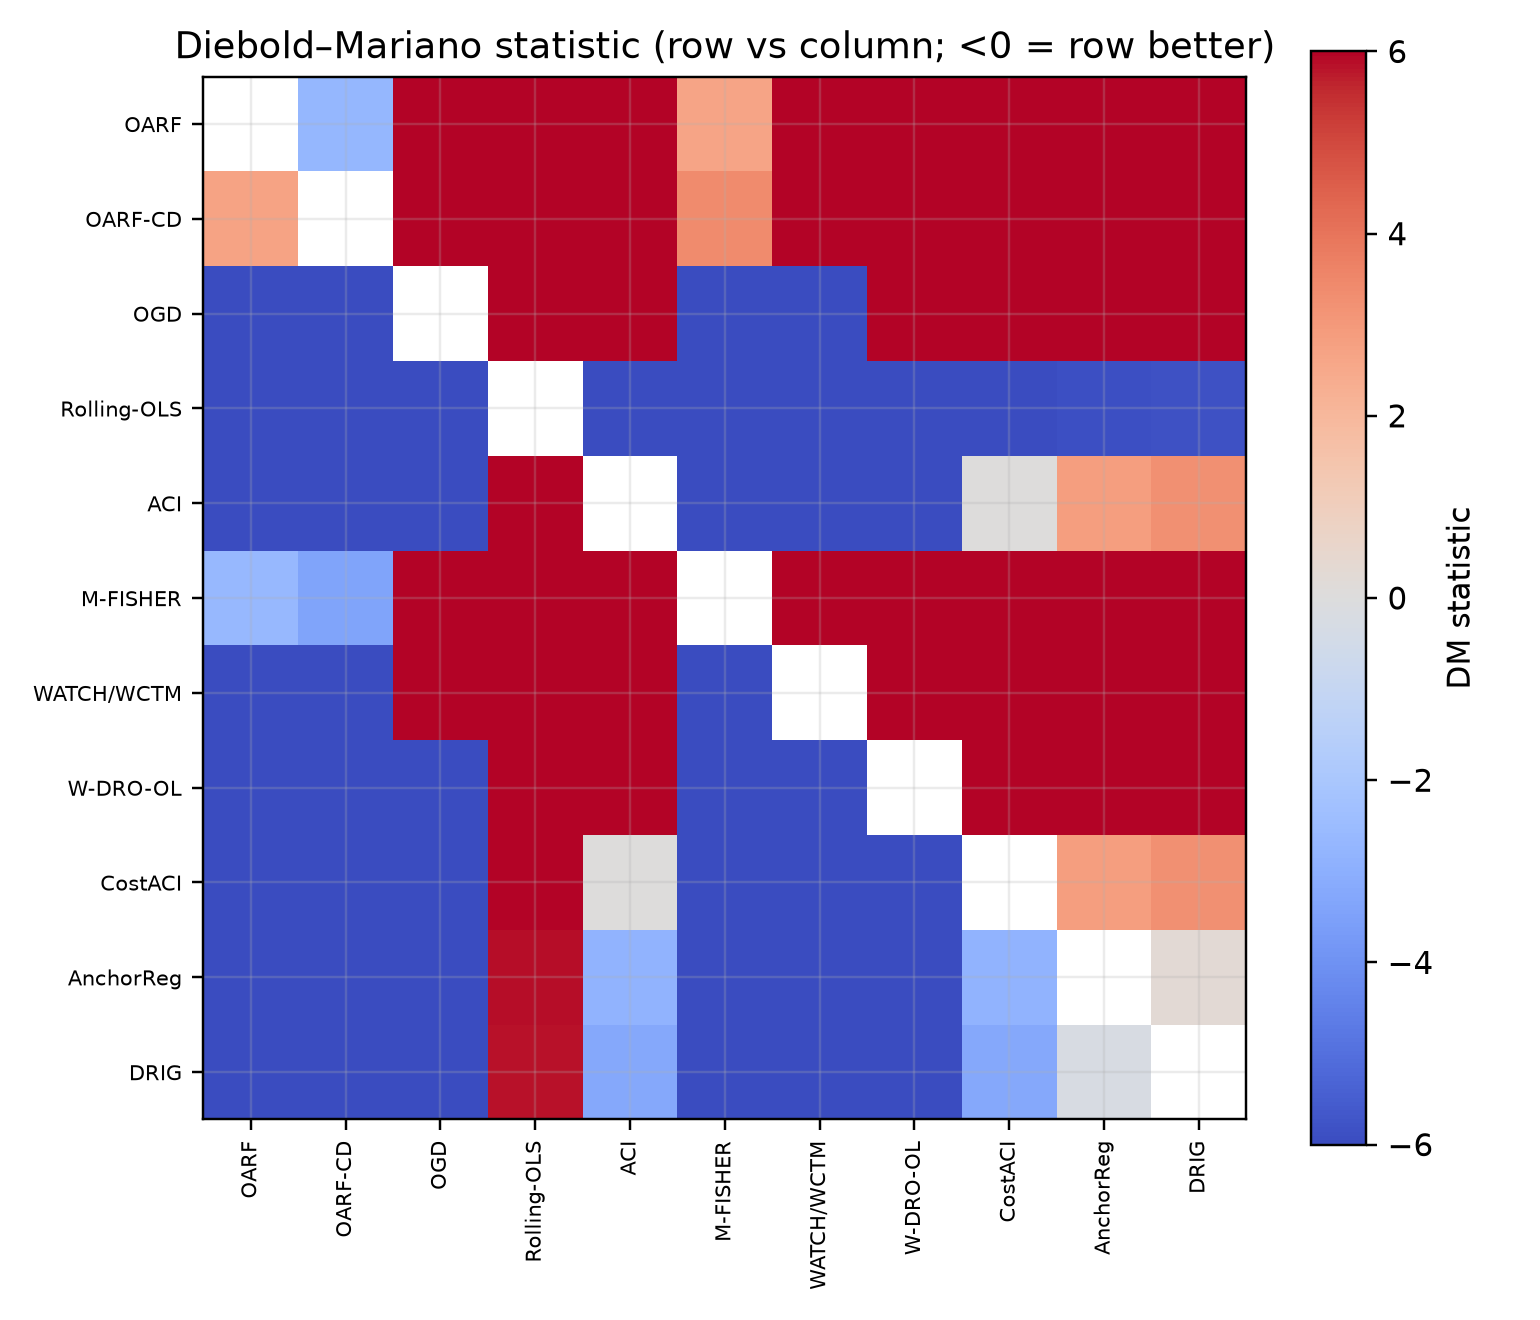
\includegraphics[width=0.62\textwidth]{fig8_dm_heatmap.png}
\caption{Pairwise Diebold--Mariano statistics on the synthetic benchmark; a negative
entry means the row method is significantly more accurate than the column method.}
\label{fig:dm}
\end{figure}

\section{Discussion and conclusion}\label{sec:discussion}

When regime shifts pass through an observable channel with anchor-mediated confounding,
a forecaster can be made robust to them in advance and online. The gain is a large
reduction in worst-case interventional error, paid for by an increase in
in-distribution error that is real but can be tuned. When that structure is weak, as on
the real energy series, the method is competitive with the strongest baselines but not
significantly better. Geometrically, distributionally robust optimisation spreads its
protection isotropically, while anchoring concentrates it on the directions in which
the regime moves. The concentration helps only to the extent that those directions are
correctly identified.

\paragraph{Scope}
The mechanism that helps under a good anchor also hurts under a bad one. \OARF{} is
likely to help when the anchor is close to exogenous, regimes are mainly mean shifts
in the anchor, the anchor is observed with at most moderate noise, and its alignment
with the true channel is above about $0.6$. It is likely to do worse than plain OGD
when the anchor is misspecified or weakly aligned, when shifts act on the target
mechanism or on the variance of the anchor, when the learned channel is unstable, or
when the stream is too short or regimes change faster than the EMA window can track. The checklist in
Section~\ref{sec:results} turns these conditions into a pre-deployment test, and for
the learned channel the eigengap $\kappa$ of Eq.~\eqref{eq:eigengap} gives an online
check; in our simulations reverting to OGD on the streams it flags cut the learned
channel's mean worst-case error by about a quarter, with a threshold set on the same
simulations.

\paragraph{Conclusion} Online anchor regression with a fixed channel gives proactive
robustness to regime shifts, backed by a fixed-anchor interventional-regret guarantee.
This holds only when the anchor behaves like an exogenous variable, is informative and
is observed with moderate noise, and only for mean-shift regimes. Outside those
conditions the method brings no benefit and can do harm. On sixteen years of daily energy variance-proxy forecasting, ten of the eleven methods lie in the Model Confidence Set, which is what our stress tests predict for a weak, noisy channel.

Online discovery of the anchor channel remains open. The block-mean rule is
reasonable but unstable, and on short data no selector does clearly better than a random channel. We made progress on a narrower
question that matters more for deployment: knowing when not to trust the discovered
channel. The eigengap diagnostic of Eq.~\eqref{eq:eigengap} is a partial
answer. It flags unreliable recovery without certifying that a well-identified subspace
is exogenous. Section~\ref{sec:results} reports the scenarios it cannot help with
(target-mechanism and variance shifts), where no channel, learned or supplied, works.
In practice, \OARF{} should be used with diagnostics: propose a candidate anchor,
validate it on a warm-up stress test, and fall back to plain online learning when the anchor, or the stability diagnostic of the discovered
channel, shows that it is weak or unstable.

The contributions are (i) a
leak-free streaming form of anchor regression with a fixed-anchor interventional-regret
guarantee; (ii) an evaluation protocol for online forecasting based on
interventional regret; (iii) a diagnostic
that needs no ground truth and lets a deployed system detect an unreliable discovered
channel and revert to plain online learning, which limits the worst-case cost of not
knowing the channel; and (iv) an empirical study of when anchor-based proactive
robustness helps or fails, with a pre-deployment checklist for deciding whether it is
appropriate for a given problem. Future work includes tightening the link between the
eigengap and a formal guarantee of robustness to misspecification, sharper online
channel discovery, nonlinear anchors and predictors, richer interventions on variances
and mechanisms, commodity-specific implied-volatility data, and event-triggered
monitoring in deployment.

\paragraph{Open theoretical question} The EMA-moment rate of $T^{2/3}$ in the
fixed-channel theorem rests, through Lemma~\ref{lem:mom}, on stationarity within regimes
(Assumption~\ref{ass:moment}). The main open problems are to tighten this rate toward
$\sqrt{T}$ without a changepoint trigger and to extend a regret guarantee to the
learned or misspecified channel. The eigengap diagnostic of Eq.~\eqref{eq:eigengap} is
a step in this direction, since Davis--Kahan already supplies the estimation-error half
of such an argument. Connecting it to a regret bound, beyond the empirical validation
reported here, remains open.

\paragraph{Reproducibility} All code and data-build scripts that regenerate every
number, table and figure in this paper will be released in a public repository upon
acceptance. For double-anonymized review the repository link is withheld from this
anonymized manuscript; it is given to the editor on the title page.
\appendix

\section{Proof of Theorem~\ref{thm:main}}\label{app:proof}
Throughout, $\mathcal{R}_t(w):=\sup_{\|\nu\|\le\rho(\xi)}\E_{\doop(a:=\nu)}
[(y_t-w^\top\phi(x_t))^2]$ is the per-step worst-case risk in \eqref{eq:intreg}, and
$\hat g_t$ is the (inexact) step direction of Algorithm~\ref{alg:oarf}.

\begin{lemma}[Convex surrogate and gradient decomposition]\label{lem:surrogate}
$\mathcal{R}_t$ is convex, and under Assumption~\ref{ass:scm} it equals, within the active
regime, the anchor-penalised risk $\mathcal{R}_t(w)=\E_t[(y-w^\top\phi)^2]+\xi P_t(w)$ of
\eqref{eq:bar}. Moreover $\hat g_t=\nabla\mathcal{R}_t(w_t)+\zeta_t$ with $\zeta_t=M_t+b_t$,
where $M_t:=-r_t\phi(x_t)-\E_t[-r\phi]$ is a martingale difference
($\E[M_t\mid\mathcal F_{t-1}]=0$) and $b_t$ is the deterministic
($\mathcal F_{t-1}$-measurable) error of the EMA-estimated penalty gradient relative to
$\nabla(\xi P_t)$.
\end{lemma}
\begin{proof}
For fixed $\nu$, $\E_{\doop(a:=\nu)}[(y-w^\top\phi)^2]$ is a convex quadratic in $w$; a
pointwise supremum of convex functions is convex. The identity is
Proposition~\ref{prop:equiv} within the stationary active regime. The prediction term
$-r_t\phi(x_t)$ is an unbiased one-sample estimate of
$\tfrac12\nabla\E_t[(y-w^\top\phi)^2]=-\E_t[r\phi]$, with centred part $M_t$; the
robustness term substitutes the $\mathcal F_{t-1}$-measurable EMA moments for the
population moments in $\nabla(\xi P_t)$, and $b_t$ is that substitution error.
\end{proof}

\begin{lemma}[Inexact dynamic regret]\label{lem:ogd}
Run projected OGD with the path-length-adaptive Ader wrapper
\citep{zhang2018adaptive} on the convex losses $\mathcal{R}_t$, fed $\hat g_t$. Then for any
$u_{1:T}\subset\mathcal{W}$ of path length $P_T$,
$\sum_t\mathcal{R}_t(w_t)-\sum_t\mathcal{R}_t(u_t)\le O(\sqrt{T(1+P_T)})+\sum_t\langle\zeta_t,
w_t-u_t\rangle$, with the first term attained without prior knowledge of $P_T$.
\end{lemma}
\begin{proof}
With exact gradients, Ader attains minimax dynamic regret $O(\sqrt{T(1+P_T)})$ for
convex $G$-Lipschitz losses over a radius-$D$ set, adaptively in $P_T$
\citep{zhang2018adaptive}, subsuming \citet{zinkevich2003ogd,hazan2016oco}. Convexity
gives $\mathcal{R}_t(w_t)-\mathcal{R}_t(u_t)\le\langle\nabla\mathcal{R}_t(w_t),w_t-u_t\rangle=
\langle\hat g_t,w_t-u_t\rangle-\langle\zeta_t,w_t-u_t\rangle$; summing and applying the
exact-gradient bound to the $\hat g_t$ terms yields the inexactness term.
\end{proof}

\begin{lemma}[Gradient-error control]\label{lem:mom}
Under Assumptions~\ref{ass:bounded}--\ref{ass:moment}, against the deterministic
minimising comparator: (i) $\E[\sum_t\langle M_t,w_t-u_t\rangle]=0$; and (ii)
$\E\|b_t\|\le c_1\sqrt{1-\beta}$ at steps at least $1/(1-\beta)$ into a regime, with
$\|b_t\|\le c_2$ within $1/(1-\beta)$ steps of each of the $K$ changes, so
$\sum_t\E\|b_t\|\le c_1 T\sqrt{1-\beta}+c_2 K/(1-\beta)$; with oracle moments $b_t\equiv0$.
\end{lemma}
\begin{proof}
(i) $w_t$ is $\mathcal F_{t-1}$-measurable and, the schedule being oblivious
(Assumption~\ref{ass:comp}), $u_t$ is deterministic, so
$\E[\langle M_t,w_t-u_t\rangle\mid\mathcal F_{t-1}]=0$; the tower rule concludes. (ii) An
EMA of decay $\beta$ of a stationary sequence has variance $\Theta(1-\beta)$ about its
mean and geometrically-decaying within-regime bias; by Assumption~\ref{ass:bounded} the
penalty gradient is Lipschitz in these moments (the $\epsilon$-ridge bounds the
inverse), inheriting the $\Theta(\sqrt{1-\beta})$ steady-state scale. After a change the
EMA mixes the previous regime for $O(1/(1-\beta))$ steps with bounded $\|b_t\|\le c_2$.
Summing gives the bound; oracle moments make the substitution error vanish.
\end{proof}

\begin{proof}[Proof of Theorem~\ref{thm:main}]
Combining the lemmas and taking expectations, for the deterministic minimiser
$u_{1:T}\in\mathcal{W}$ ($P_T\le 2DK$),
$\E[\sum_t\mathcal{R}_t(w_t)]-\sum_t\mathcal{R}_t(u_t)\le O(\sqrt{T(1+K)})+0+D\sum_t\E\|b_t\|$.
With oracle moments the last term vanishes, giving (i); with EMA moments it is
$\le D(c_1T\sqrt{1-\beta}+c_2K/(1-\beta))$, which at $1-\beta_T=T^{-2/3}$ is
$O((1+K)T^{2/3})$ and dominates $\sqrt{T(1+K)}$, giving (ii). Finally, by
Assumption~\ref{ass:scm} the realised regime is an admissible intervention, so
$\E_t[\ell_t(w_t)\mid\mathcal F_{t-1}]\le\mathcal{R}_t(w_t)$ and hence
$\E[\sum_t\ell_t(w_t)]\le\E[\sum_t\mathcal{R}_t(w_t)]$; as
$\min_{u\in\mathcal{W}}\sum_t\mathcal{R}_t(u)$ is the comparator in \eqref{eq:intreg}, the
displays bound $\E[\mathrm{IntReg}_T(\rho(\xi))]$ by the stated rates.
\end{proof}

\section{Decision-economic evaluation (secondary)}\label{app:econ}
As a secondary check we convert each method's volatility forecast into a
volatility-timing portfolio \citep{fleming2001voltiming}. Exposure is scaled inversely
to the forecast variance, $w_t=\mathrm{clip}(\sigma^\star{}^2/\hat\sigma_t^2,0,3)$, and
the strategy earns $w_t r_{t+1}$ net of a one-basis-point turnover cost. We report the
annualised Sharpe ratio, maximum drawdown and turnover. Over 2010--2026 the Sharpe ratios
of these commodity risk-targeting strategies are low and statistically indistinguishable
across methods (Figure~\ref{fig:equity}). The evaluation is reported for completeness
only; it carries no evidential weight, and no claim in the main text rests on it.

\begin{figure}[htbp]
\centering
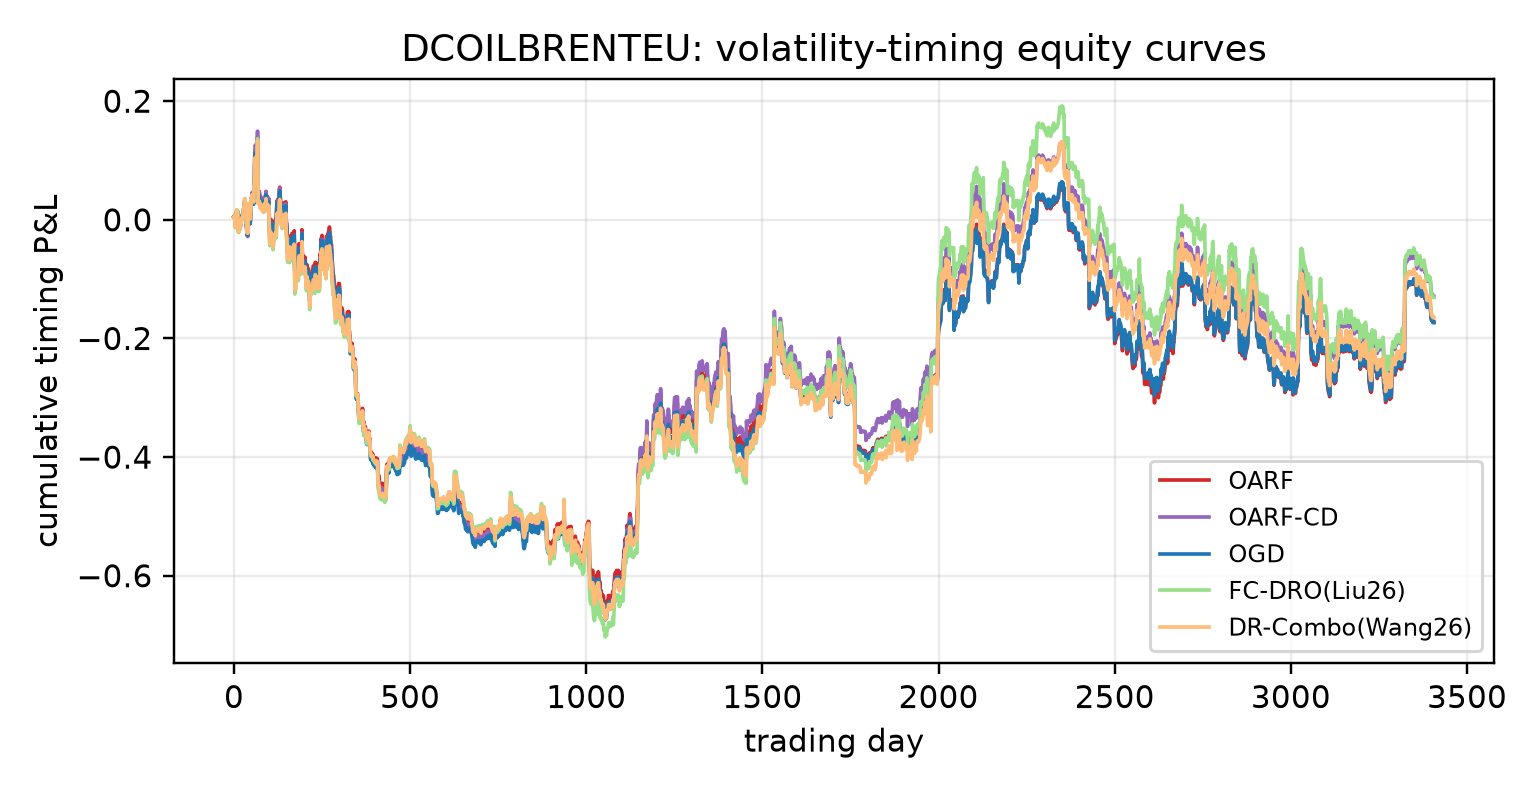
\includegraphics[width=0.66\textwidth]{fig10_equity_DCOILBRENTEU.png}
\caption{Brent: cumulative volatility-timing profit and loss. Differences across methods
are economically small and not statistically significant over this sample.}
\label{fig:equity}
\end{figure}

\section{Baseline implementations and notes}\label{app:baselines}
Table~\ref{tab:baseimpl} lists, for each method, the loss optimised, the update rule
and the output, whether the method runs online, rolling or in batch, and whether it uses
the anchor. All methods run under the same leak-free protocol with the hyper-parameters
of Table~\ref{tab:hyper}. Per step, the linear methods cost $O(d)$ and \OARF{} adds
$O(pq+q^3)$ for the anchor block. Rolling-OLS and the batch methods cost $O(d^3)$ at
each refit, which takes place every $5$--$10$ steps.

Some implementation details follow. The warm-up block is used only to initialise the
past-only standardiser and to select hyper-parameters once; it is never used for
separate batch pre-training. Missing FRED observations and exchange holidays are
handled by reindexing to business days with a forward-fill capped at five days, and
longer gaps are left missing and skipped. After the warm-up the GARCH$(1,1)$ expert
keeps fixed RiskMetrics-style coefficients and is not re-estimated online, so it is a
fixed-parameter recursion. The channel dimension is larger on the real data ($q=3$,
against $q=2$ in the synthetic experiments) because three macro-uncertainty drivers
(VIX, GPR, EPU) are chosen by hand as the anchor, while the synthetic SCM has exactly
two anchor directions by construction. We present \OARF{} for linear predictors. It
extends to nonlinear forecasters by applying the same residual--anchor penalty to a
feature map or to the top layer of a network; we leave this extension to future work.

\begin{table}[htbp]
\centering
\caption{Baseline implementations. ``Out'' = P(oint)/I(nterval); ``Mode'' =
O(nline)/R(olling)/B(atch); ``Anc'' = uses the anchor.}
\label{tab:baseimpl}
\small
\begin{tabular}{lllccc}
\toprule
Method & Loss optimised & Update rule & Out & Mode & Anc\\
\midrule
\OARF{}/\OARFCD{} & anchor-penalised sq.\ err. & AdaGrad on \eqref{eq:update} & P & O & yes\\
OGD & squared error & AdaGrad ($\xi=0$) & P & O & no\\
Rolling-OLS & windowed ridge & closed-form refit & P & R & no\\
ACI/CostACI & pinball (3 quantiles) & subgrad.\ + ACI level & P+I & O & no\\
M-FISHER & sq.\ err.\ + martingale & OGD + triggered NGD & P & O & no\\
WATCH/WCTM & sq.\ err.\ + WCTM & OGD + width adapt & P+I & O & no\\
DR-Combo & Wasserstein-DR combo & EG mirror descent & P & O & no\\
FC-DRO(-ES) & variance-/ES-scaled & exponential weights & P & O & no\\
W-DRO-OL & Wasserstein-DR sq.\ err. & primal--dual OGD & P & O & no\\
AnchorReg & anchor-penalised (batch) & windowed closed-form & P & R & yes\\
DRIG & invariant-gradient (batch) & windowed two-env.\ fit & P & R & (env)\\
\bottomrule
\end{tabular}
\end{table}

\section{Ader-wrapped versus AdaGrad OARF}\label{app:ader}
The interventional-regret theorem (Theorem~\ref{thm:main}) is stated for the
path-length-adaptive Ader step wrapper \citep{zhang2018adaptive}, whereas the deployed
model takes a single AdaGrad step. To check whether this simplification changes the
empirical behaviour, we implemented the Ader variant and compared it with the deployed
AdaGrad model on the controlled anchor-SCM (true fixed channel, $\xi=6$, $12$ seeds).
The Ader variant is a pool of five gradient-descent experts that follow the same
anchor-robust surrogate gradient with a geometric ladder of step sizes. Each expert is
projected onto the comparator ball, and a Hedge meta-learner combines them.
Table~\ref{tab:ader} reports the results. Both step rules cut the worst-case $\doop(A)$ error well below the no-anchor OGD reference, to about a third (AdaGrad) and a half (Ader) of it, and their per-seed worst-case
errors are strongly rank-correlated (Spearman $\rho=0.80$). In this experiment AdaGrad
is slightly more accurate and has lower variance. It also has fewer parameters, and for
these reasons it is the rule we deploy; the Ader wrapper is the object the theorem
analyses. Substituting one for the other leaves the qualitative ranking unchanged.

\begin{table}[htbp]
\centering
\caption{Ader-wrapped versus AdaGrad \OARF{} on the synthetic anchor-SCM ($12$ seeds,
true fixed channel, $\xi=6$; median with $[\,q_{25},q_{75}\,]$). Both reach similar
worst-case interventional error, far below the OGD reference, and their per-seed worst-case
errors are rank-correlated at Spearman $\rho=0.80$.}
\label{tab:ader}
\small
\begin{tabular}{lcc}
\toprule
Step rule & in-regime MSE & worst-$\doop(A)$ MSE\\
\midrule
AdaGrad (deployed) & $0.028$ & $0.052\,[0.030,0.114]$\\
Ader (analysed)    & $0.030$ & $0.073\,[0.026,0.142]$\\
\midrule
OGD ($\xi=0$, reference) & $0.019$ & $0.143\,[0.065,0.353]$\\
\bottomrule
\end{tabular}
\end{table}

\section{Event study: COVID-19 and the 2022 energy shock}\label{app:events}
The regime-tercile analysis in the main text is aggregate, so here we examine two dated
episodes. We run fixed-anchor \OARF{} ($\xi=1.5$) and the no-anchor OGD reference on the
real combination stream. Within each event window we plot the cumulative squared-loss
gap (\OARF{} minus OGD, so a negative value means \OARF{} is ahead) and, for both
methods, the smoothed anchor--residual correlation $|\mathrm{corr}(a_t,r_t)|$
(Figure~\ref{fig:events}). In every window \OARF{} keeps the anchor--residual
correlation visibly below that of OGD, so on real data the update does what it is
designed to do. This does not produce a consistent loss advantage. \OARF{} is ahead
during the COVID-19 window on Brent (cumulative squared-loss gap $-0.27$) and behind in
the other three window/commodity combinations (gaps of $+0.30$ to $+1.58$). The pattern
matches the Model-Confidence-Set result: on this public daily data the anchor mechanism
is active, but it is too weakly coupled to the target to give a dependable forecasting
edge. The event study illustrates this around recognisable episodes; it does not
demonstrate that \OARF{} is superior.

\begin{figure}[htbp]
\centering
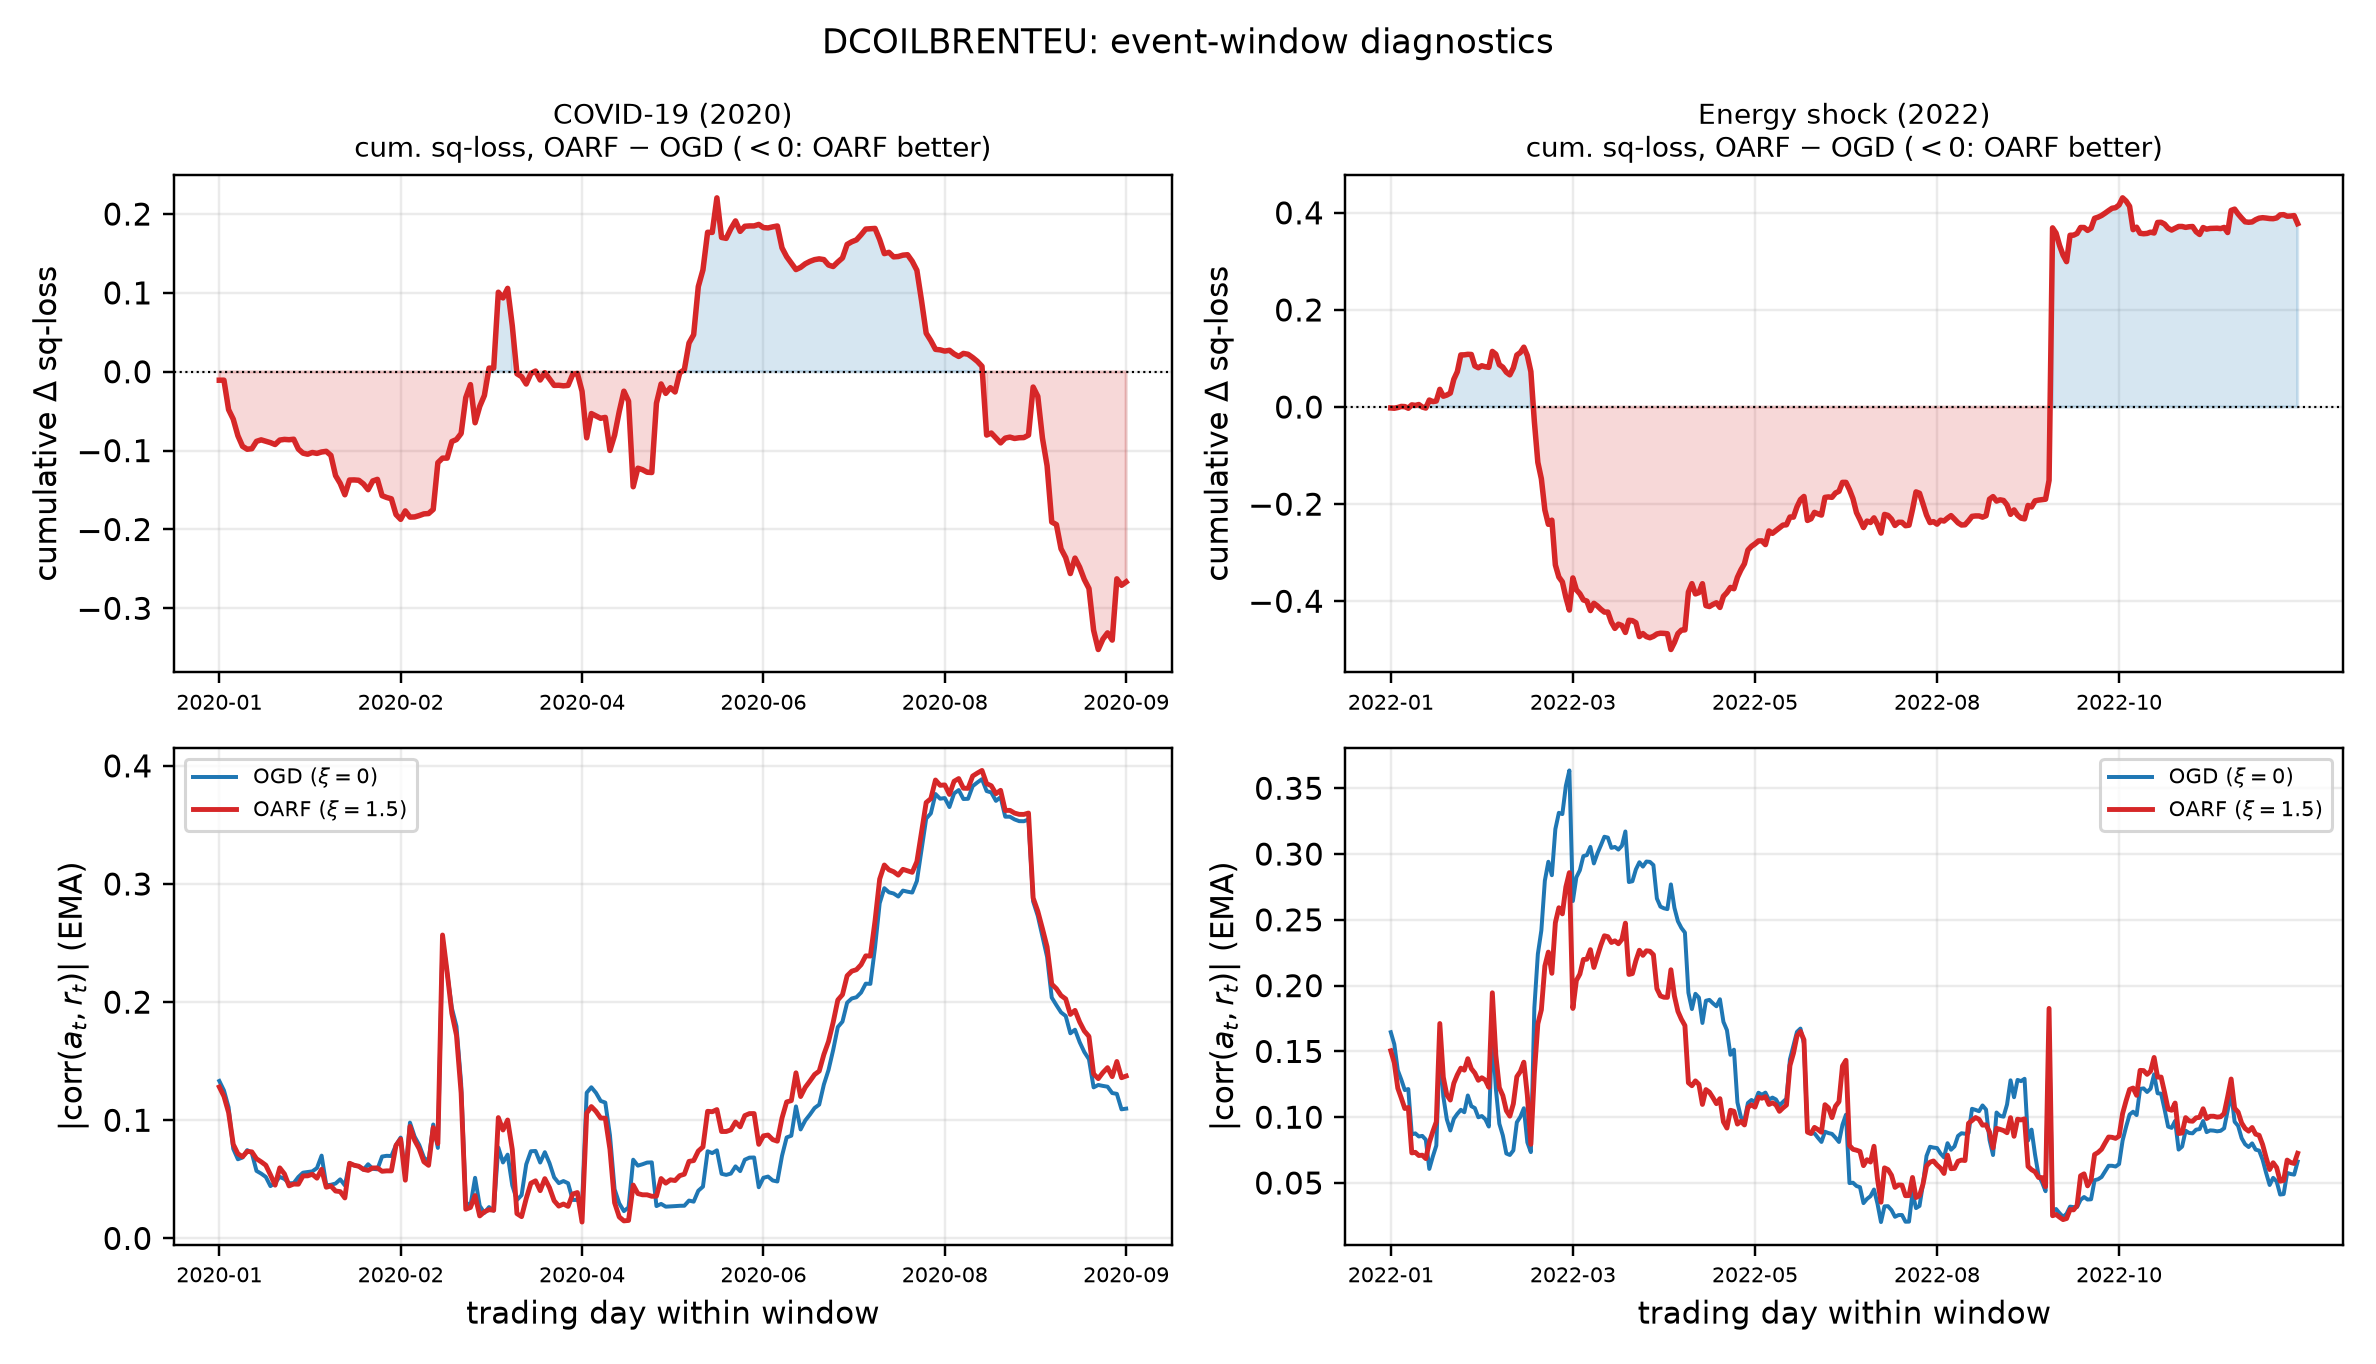
\includegraphics[width=0.96\textwidth]{fig15_events_DCOILBRENTEU.png}
\caption{Brent event windows. Top: cumulative squared-loss gap, \OARF{} minus OGD
(shaded blue where \OARF{} leads, orange where it trails). Bottom: the smoothed
anchor--residual correlation, which \OARF{} holds below OGD in both windows. \OARF{}
leads during the 2020 COVID-19 crash but trails during the 2022 energy shock,
consistent with the statistically insignificant aggregate result.}
\label{fig:events}
\end{figure}

\section*{Funding}
This research did not receive any specific grant from funding agencies in the
public, commercial, or not-for-profit sectors.

\section*{Declaration of competing interest}
The author declares that he has no known competing financial interests or
personal relationships that could have appeared to influence the work reported
in this paper.

\section*{CRediT authorship contribution statement}
The corresponding author is responsible for conceptualization, methodology,
software, formal analysis, investigation, data curation, writing (original
draft, review and editing), and visualization.

\section*{Data availability}
Public data sources and the code that regenerates every number, table and
figure in this paper (see Reproducibility, above) will be made available in a
public repository upon acceptance.

\section*{Declaration of generative AI and AI-assisted technologies in the manuscript preparation process}
During the preparation of this work, the author used an AI-based writing
assistant to help draft and revise text and improve the clarity of exposition,
following the author's direction and intent. After using this tool, the
author reviewed, verified and edited all content and takes full
responsibility for the content of the published article.

\small
\bibliographystyle{elsarticle-harv}
\bibliography{references}

\end{document}
